% Options for packages loaded elsewhere
\PassOptionsToPackage{unicode}{hyperref}
\PassOptionsToPackage{hyphens}{url}
\documentclass[
]{article}
\usepackage{xcolor}
\usepackage{amsmath,amssymb}
\setcounter{secnumdepth}{-\maxdimen} % remove section numbering
\usepackage{iftex}
\ifPDFTeX
  \usepackage[T1]{fontenc}
  \usepackage[utf8]{inputenc}
  \usepackage{textcomp} % provide euro and other symbols
\else % if luatex or xetex
  \usepackage{unicode-math} % this also loads fontspec
  \defaultfontfeatures{Scale=MatchLowercase}
  \defaultfontfeatures[\rmfamily]{Ligatures=TeX,Scale=1}
\fi
\usepackage{lmodern}
\ifPDFTeX\else
  % xetex/luatex font selection
\fi
% Use upquote if available, for straight quotes in verbatim environments
\IfFileExists{upquote.sty}{\usepackage{upquote}}{}
\IfFileExists{microtype.sty}{% use microtype if available
  \usepackage[]{microtype}
  \UseMicrotypeSet[protrusion]{basicmath} % disable protrusion for tt fonts
}{}
\makeatletter
\@ifundefined{KOMAClassName}{% if non-KOMA class
  \IfFileExists{parskip.sty}{%
    \usepackage{parskip}
  }{% else
    \setlength{\parindent}{0pt}
    \setlength{\parskip}{6pt plus 2pt minus 1pt}}
}{% if KOMA class
  \KOMAoptions{parskip=half}}
\makeatother
\usepackage{longtable,booktabs,array}
\usepackage{calc} % for calculating minipage widths
% Correct order of tables after \paragraph or \subparagraph
\usepackage{etoolbox}
\makeatletter
\patchcmd\longtable{\par}{\if@noskipsec\mbox{}\fi\par}{}{}
\makeatother
% Allow footnotes in longtable head/foot
\IfFileExists{footnotehyper.sty}{\usepackage{footnotehyper}}{\usepackage{footnote}}
\makesavenoteenv{longtable}
\usepackage{graphicx}
\makeatletter
\newsavebox\pandoc@box
\newcommand*\pandocbounded[1]{% scales image to fit in text height/width
  \sbox\pandoc@box{#1}%
  \Gscale@div\@tempa{\textheight}{\dimexpr\ht\pandoc@box+\dp\pandoc@box\relax}%
  \Gscale@div\@tempb{\linewidth}{\wd\pandoc@box}%
  \ifdim\@tempb\p@<\@tempa\p@\let\@tempa\@tempb\fi% select the smaller of both
  \ifdim\@tempa\p@<\p@\scalebox{\@tempa}{\usebox\pandoc@box}%
  \else\usebox{\pandoc@box}%
  \fi%
}
% Set default figure placement to htbp
\def\fps@figure{htbp}
\makeatother
\setlength{\emergencystretch}{3em} % prevent overfull lines
\providecommand{\tightlist}{%
  \setlength{\itemsep}{0pt}\setlength{\parskip}{0pt}}
\usepackage{bookmark}
\IfFileExists{xurl.sty}{\usepackage{xurl}}{} % add URL line breaks if available
\urlstyle{same}
\hypersetup{
  hidelinks,
  pdfcreator={LaTeX via pandoc}}

\author{}
\date{}

\begin{document}

OptiVest AI: An Explainable AI-Driven Autonomous Wealth Management
Platform with Intelligent Portfolio Reallocation

Naitik Pathak Department of Computer Science / Quantitative Finance
Independent Research

\textbf{\emph{Abstract}}---\textbf{Modern quantitative wealth management
systems consistently face two profound challenges that hinder their
adoption in retail and regulated environments. First, they suffer from
the Prediction Fallacy, wherein stock return forecasting is treated as a
direct proxy for actionable trading decisions. Standard price
predictions fundamentally ignore vital real-world constraints such as
portfolio covariance, dynamic risk budgeting, strict user-defined
limitations, and the compounding penalty of transaction turnover.
Second, the deployment of advanced ensemble machine learning models
introduces the Black-Box Dilemma. These highly complex models recommend
portfolio reallocations without interpretable, deterministic
explanations, rendering them unacceptable for regulated applications and
eroding investor trust.}

\textbf{OptiVest AI addresses both challenges via a comprehensive
Adaptive Portfolio Decision Engine (APDE). The core historical
evaluation demonstrates the APDE's performance. The platform
additionally incorporates a Candidate Discovery Engine (CDE) for asset
pre-filtering and a TreeSHAP-based feature attribution module for
transparent explanations; these components are evaluated separately from
the original historical APDE experiment.}

\textbf{\emph{Index Terms}}---\textbf{Machine Learning, Portfolio
Optimization, Explainable AI, SHAP, Algorithmic Trading, FinTech.}

\section{OptiVest AI: An Explainable AI-Driven Autonomous Wealth
Management Platform with Intelligent Portfolio
Reallocation}\label{optivest-ai-an-explainable-ai-driven-autonomous-wealth-management-platform-with-intelligent-portfolio-reallocation}

\textbf{Abstract} Traditional quantitative wealth management systems
generally suffer from two core limitations: 1. \textbf{The Prediction
Fallacy}: Treating stock return forecasting as a direct proxy for
trading decisions. Standard price predictions ignore portfolio
covariance, portfolio risk budgeting, user constraints, and transaction
turnover penalties. 2. \textbf{The Black-Box Dilemma}: Deep learning or
ensemble ML models recommend trades without interpretable explanations,
rendering them unacceptable for regulated FinTech applications and
retail investor trust.

\textbf{OptiVest AI} addresses both challenges via a comprehensive
\textbf{Adaptive Portfolio Decision Engine (APDE)} coupled with a
\textbf{Candidate Discovery Engine (CDE)} and \textbf{TreeSHAP} feature
attribution. This paper details the mathematical foundation, system
architecture, and operational workflows of the OptiVest platform.

\begin{center}\rule{0.5\linewidth}{0.5pt}\end{center}

\subsection{1. System Architecture}\label{system-architecture}

OptiVest is designed as an end-to-end multi-dimensional investment
intelligence platform. It ingests market and fundamental signals,
pre-filters the universe through a candidate discovery phase, and
ultimately generates mathematically optimal and explainable allocation
decisions.

\begin{figure}
\centering
\pandocbounded{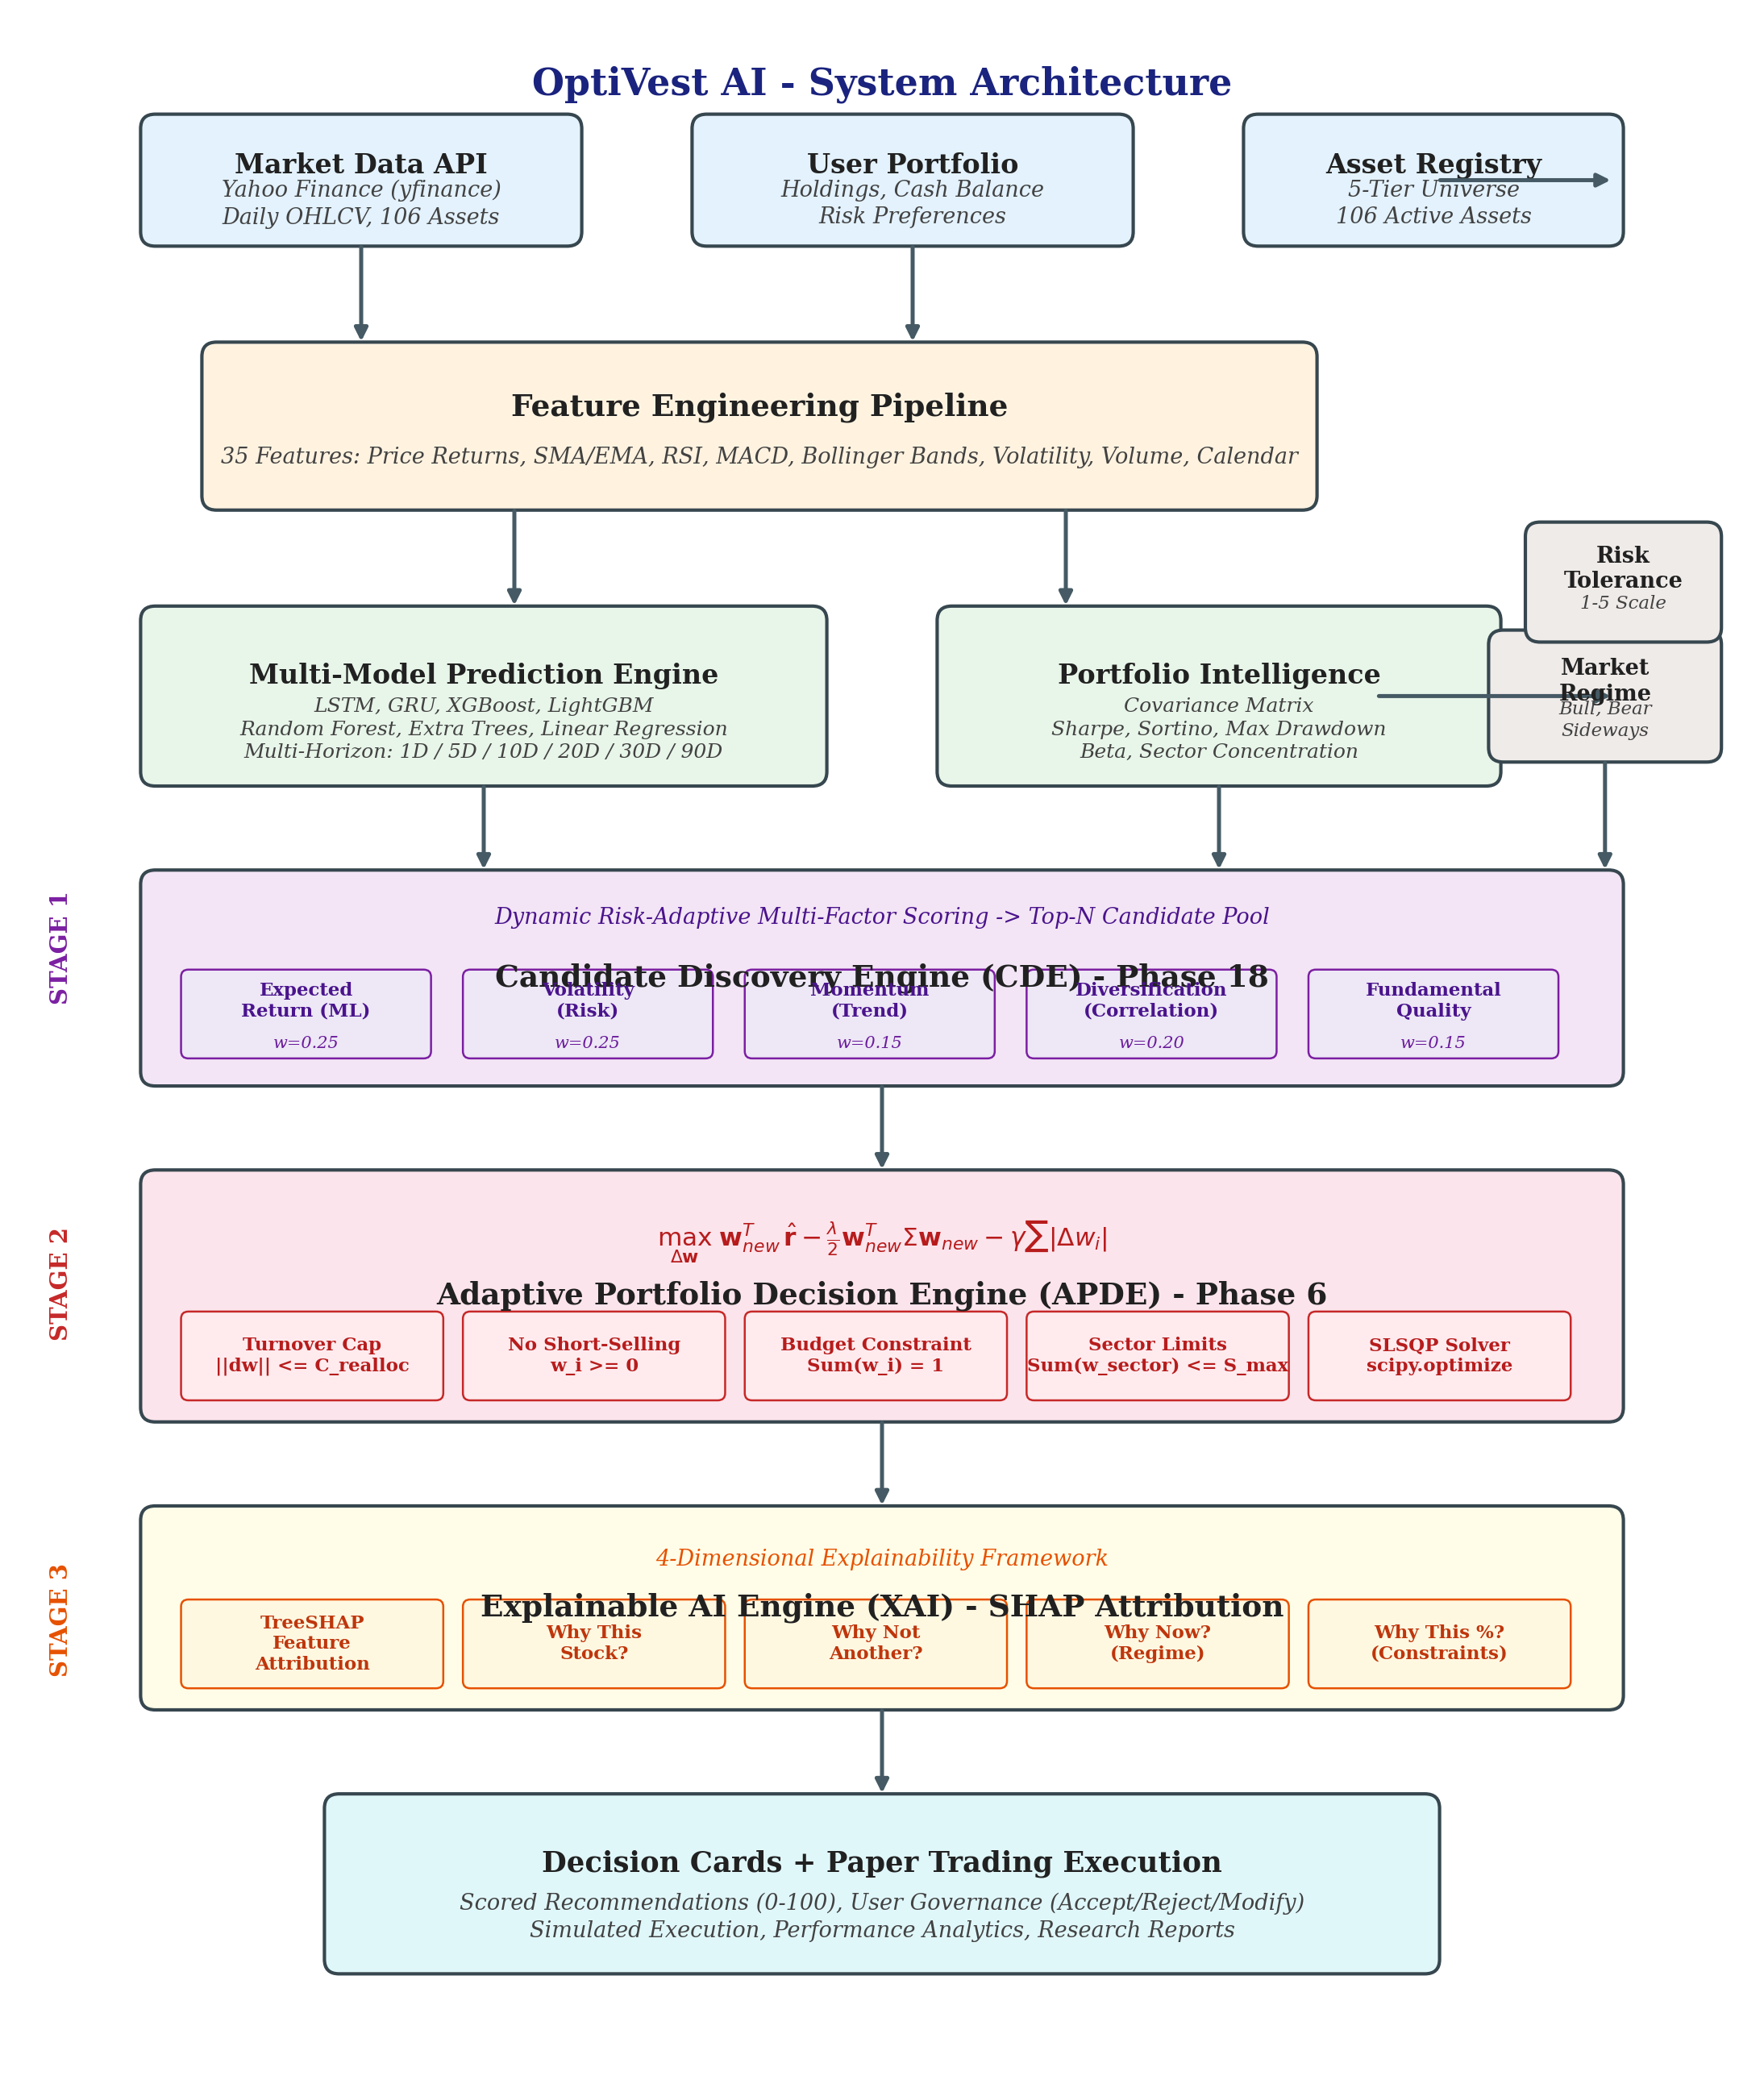
\includegraphics[keepaspectratio,alt={System Architecture}]{./figures/output/fig01_system_architecture.png}}
\caption{System Architecture}
\end{figure}

The system operates across several layers: - \textbf{Data Ingestion}:
Yahoo Finance serves as the primary provider for both real-time market
prices and current-snapshot fundamental financial statements. -
\textbf{Intelligence Layer}: Combines XGBoost predictive models,
statistical covariance analysis, and fundamental quality scoring. -
\textbf{Decision Engine (APDE)}: A multi-objective optimizer that
translates signals into compliant portfolio weights. -
\textbf{Explainability (XAI)}: SHAP-based narrations demystify the
``why'' behind every trade.

\begin{center}\rule{0.5\linewidth}{0.5pt}\end{center}

\subsection{2. Data Pipeline \& Asset
Universe}\label{data-pipeline-asset-universe}

Before any optimization can occur, the system defines a robust universe
of assets and processes the raw data.

\begin{figure}
\centering
\pandocbounded{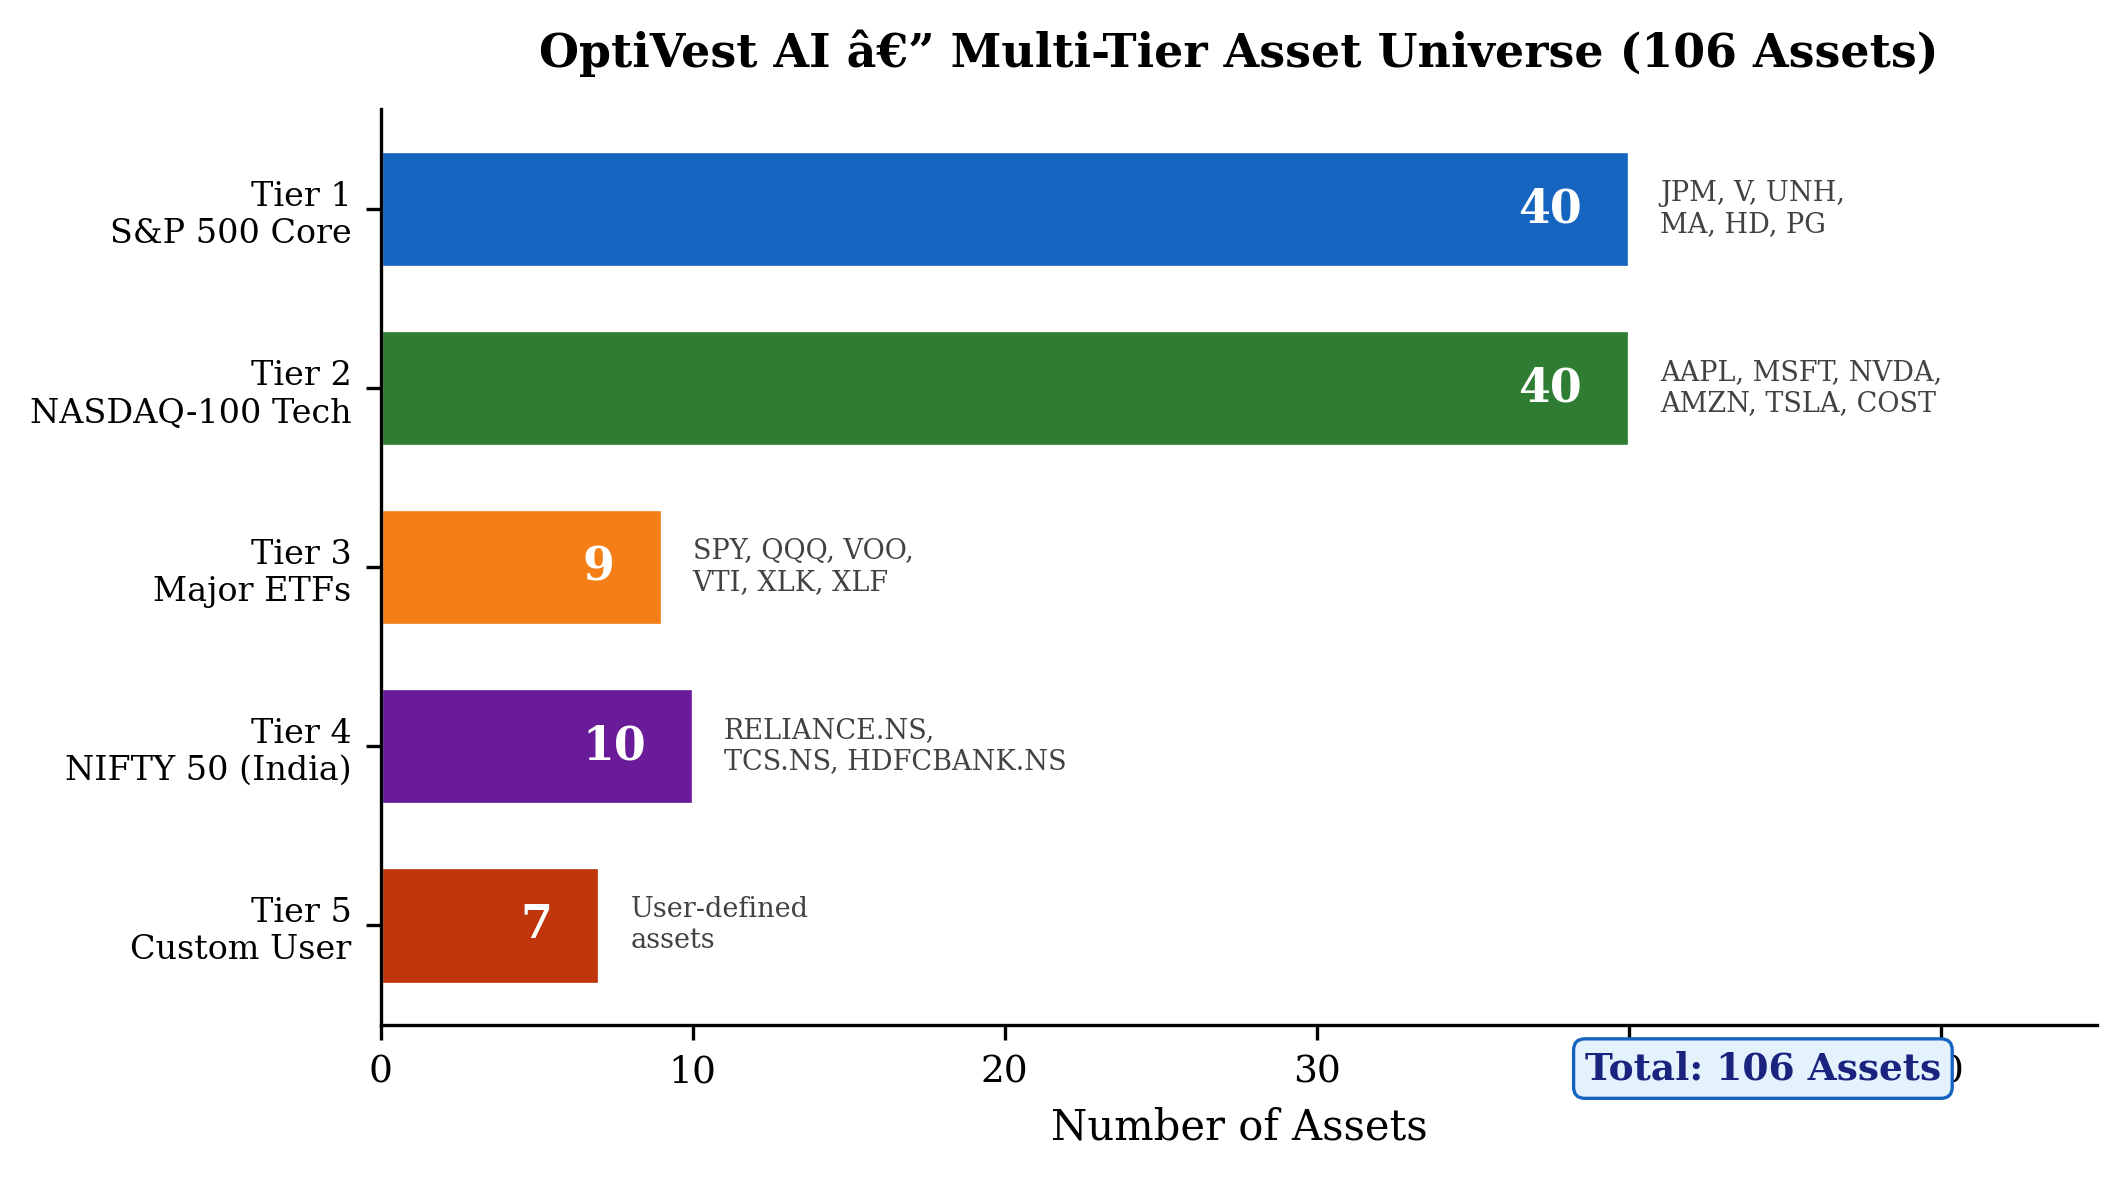
\includegraphics[keepaspectratio,alt={Asset Universe}]{./figures/output/fig02_asset_universe.png}}
\caption{Asset Universe}
\end{figure}

The data pipeline rigorously splits data chronologically to prevent
look-ahead bias during model training and evaluation.

\begin{figure}
\centering
\pandocbounded{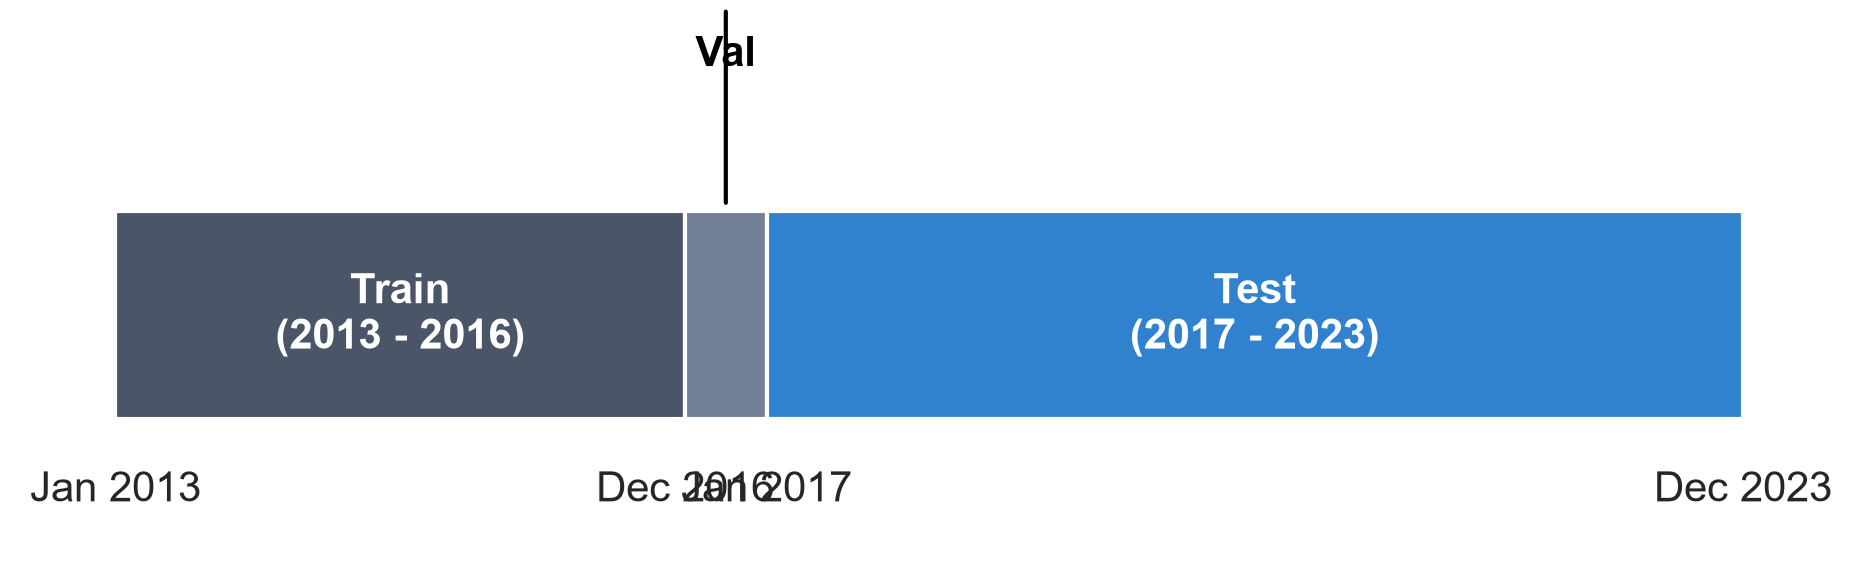
\includegraphics[keepaspectratio,alt={Data Split Strategy}]{./figures/output/fig03_data_split.png}}
\caption{Data Split Strategy}
\end{figure}

Raw financial time-series data is inherently noisy. A structured
preprocessing pipeline cleans, scales, and engineers features across a
diverse taxonomy (price momentum, volatility, volume, and macroeconomic
indicators).

\pandocbounded{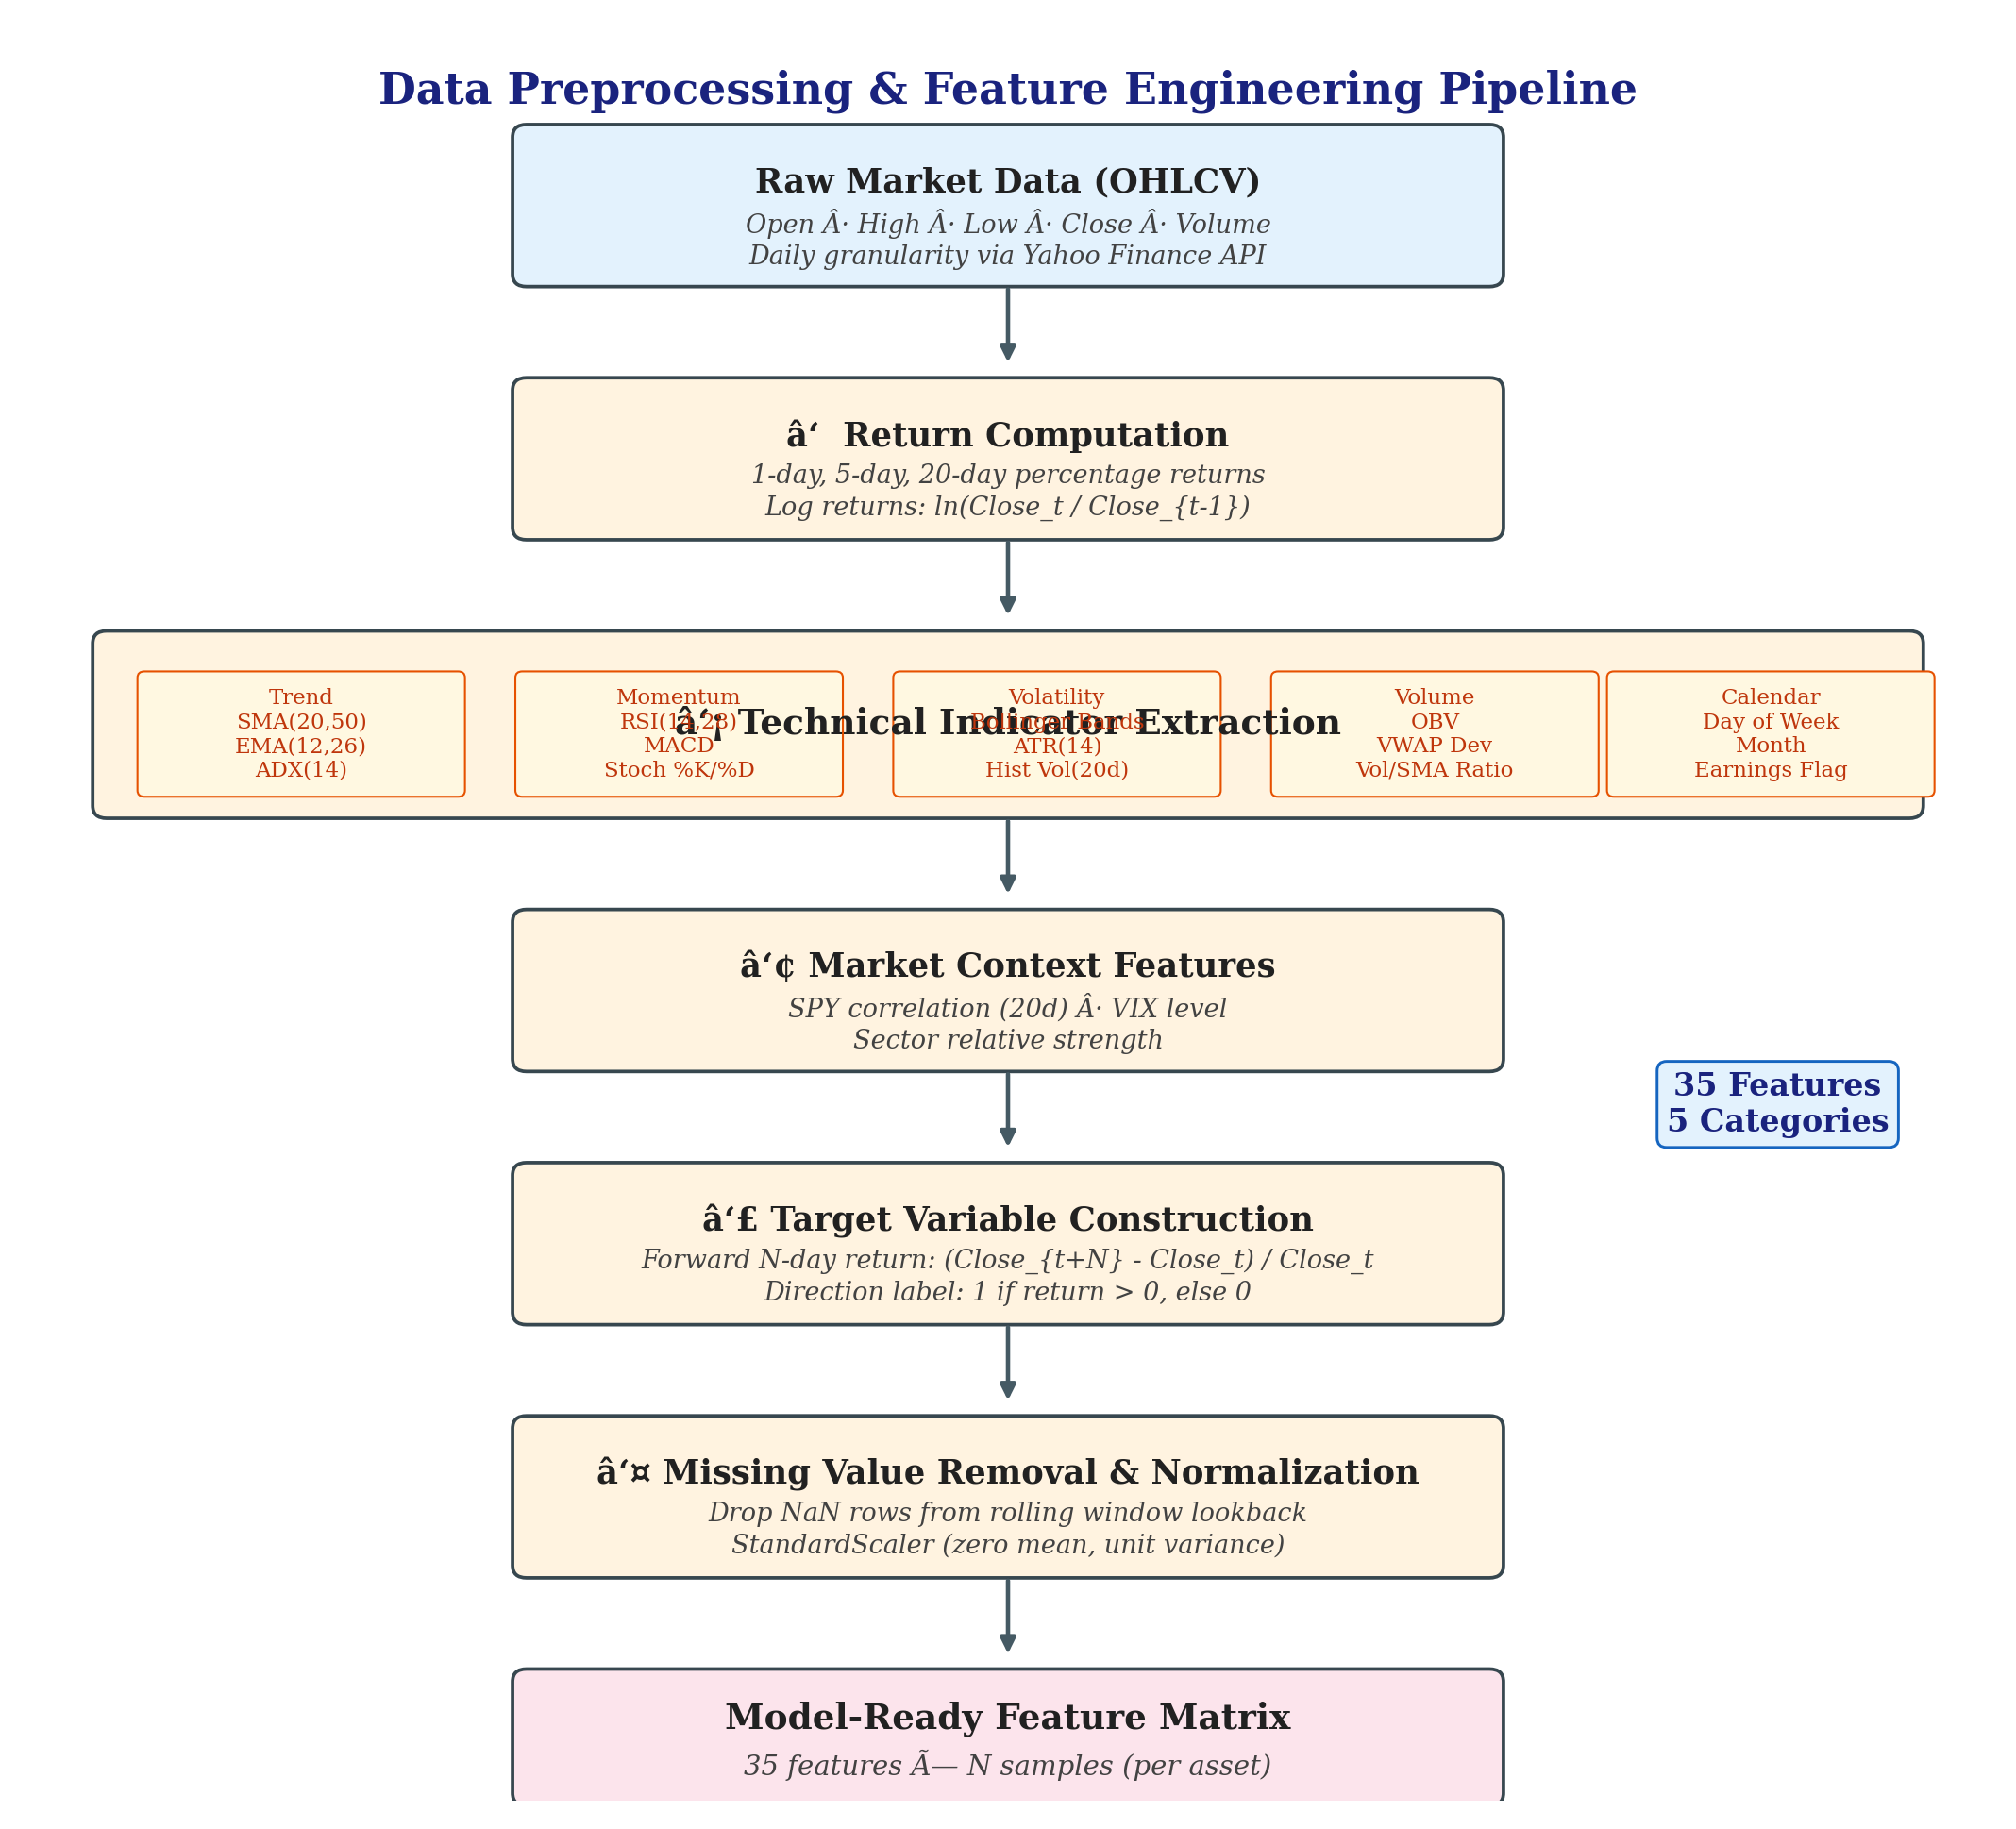
\includegraphics[keepaspectratio,alt={Preprocessing Pipeline}]{./figures/output/fig04_preprocessing_pipeline.png}}
\pandocbounded{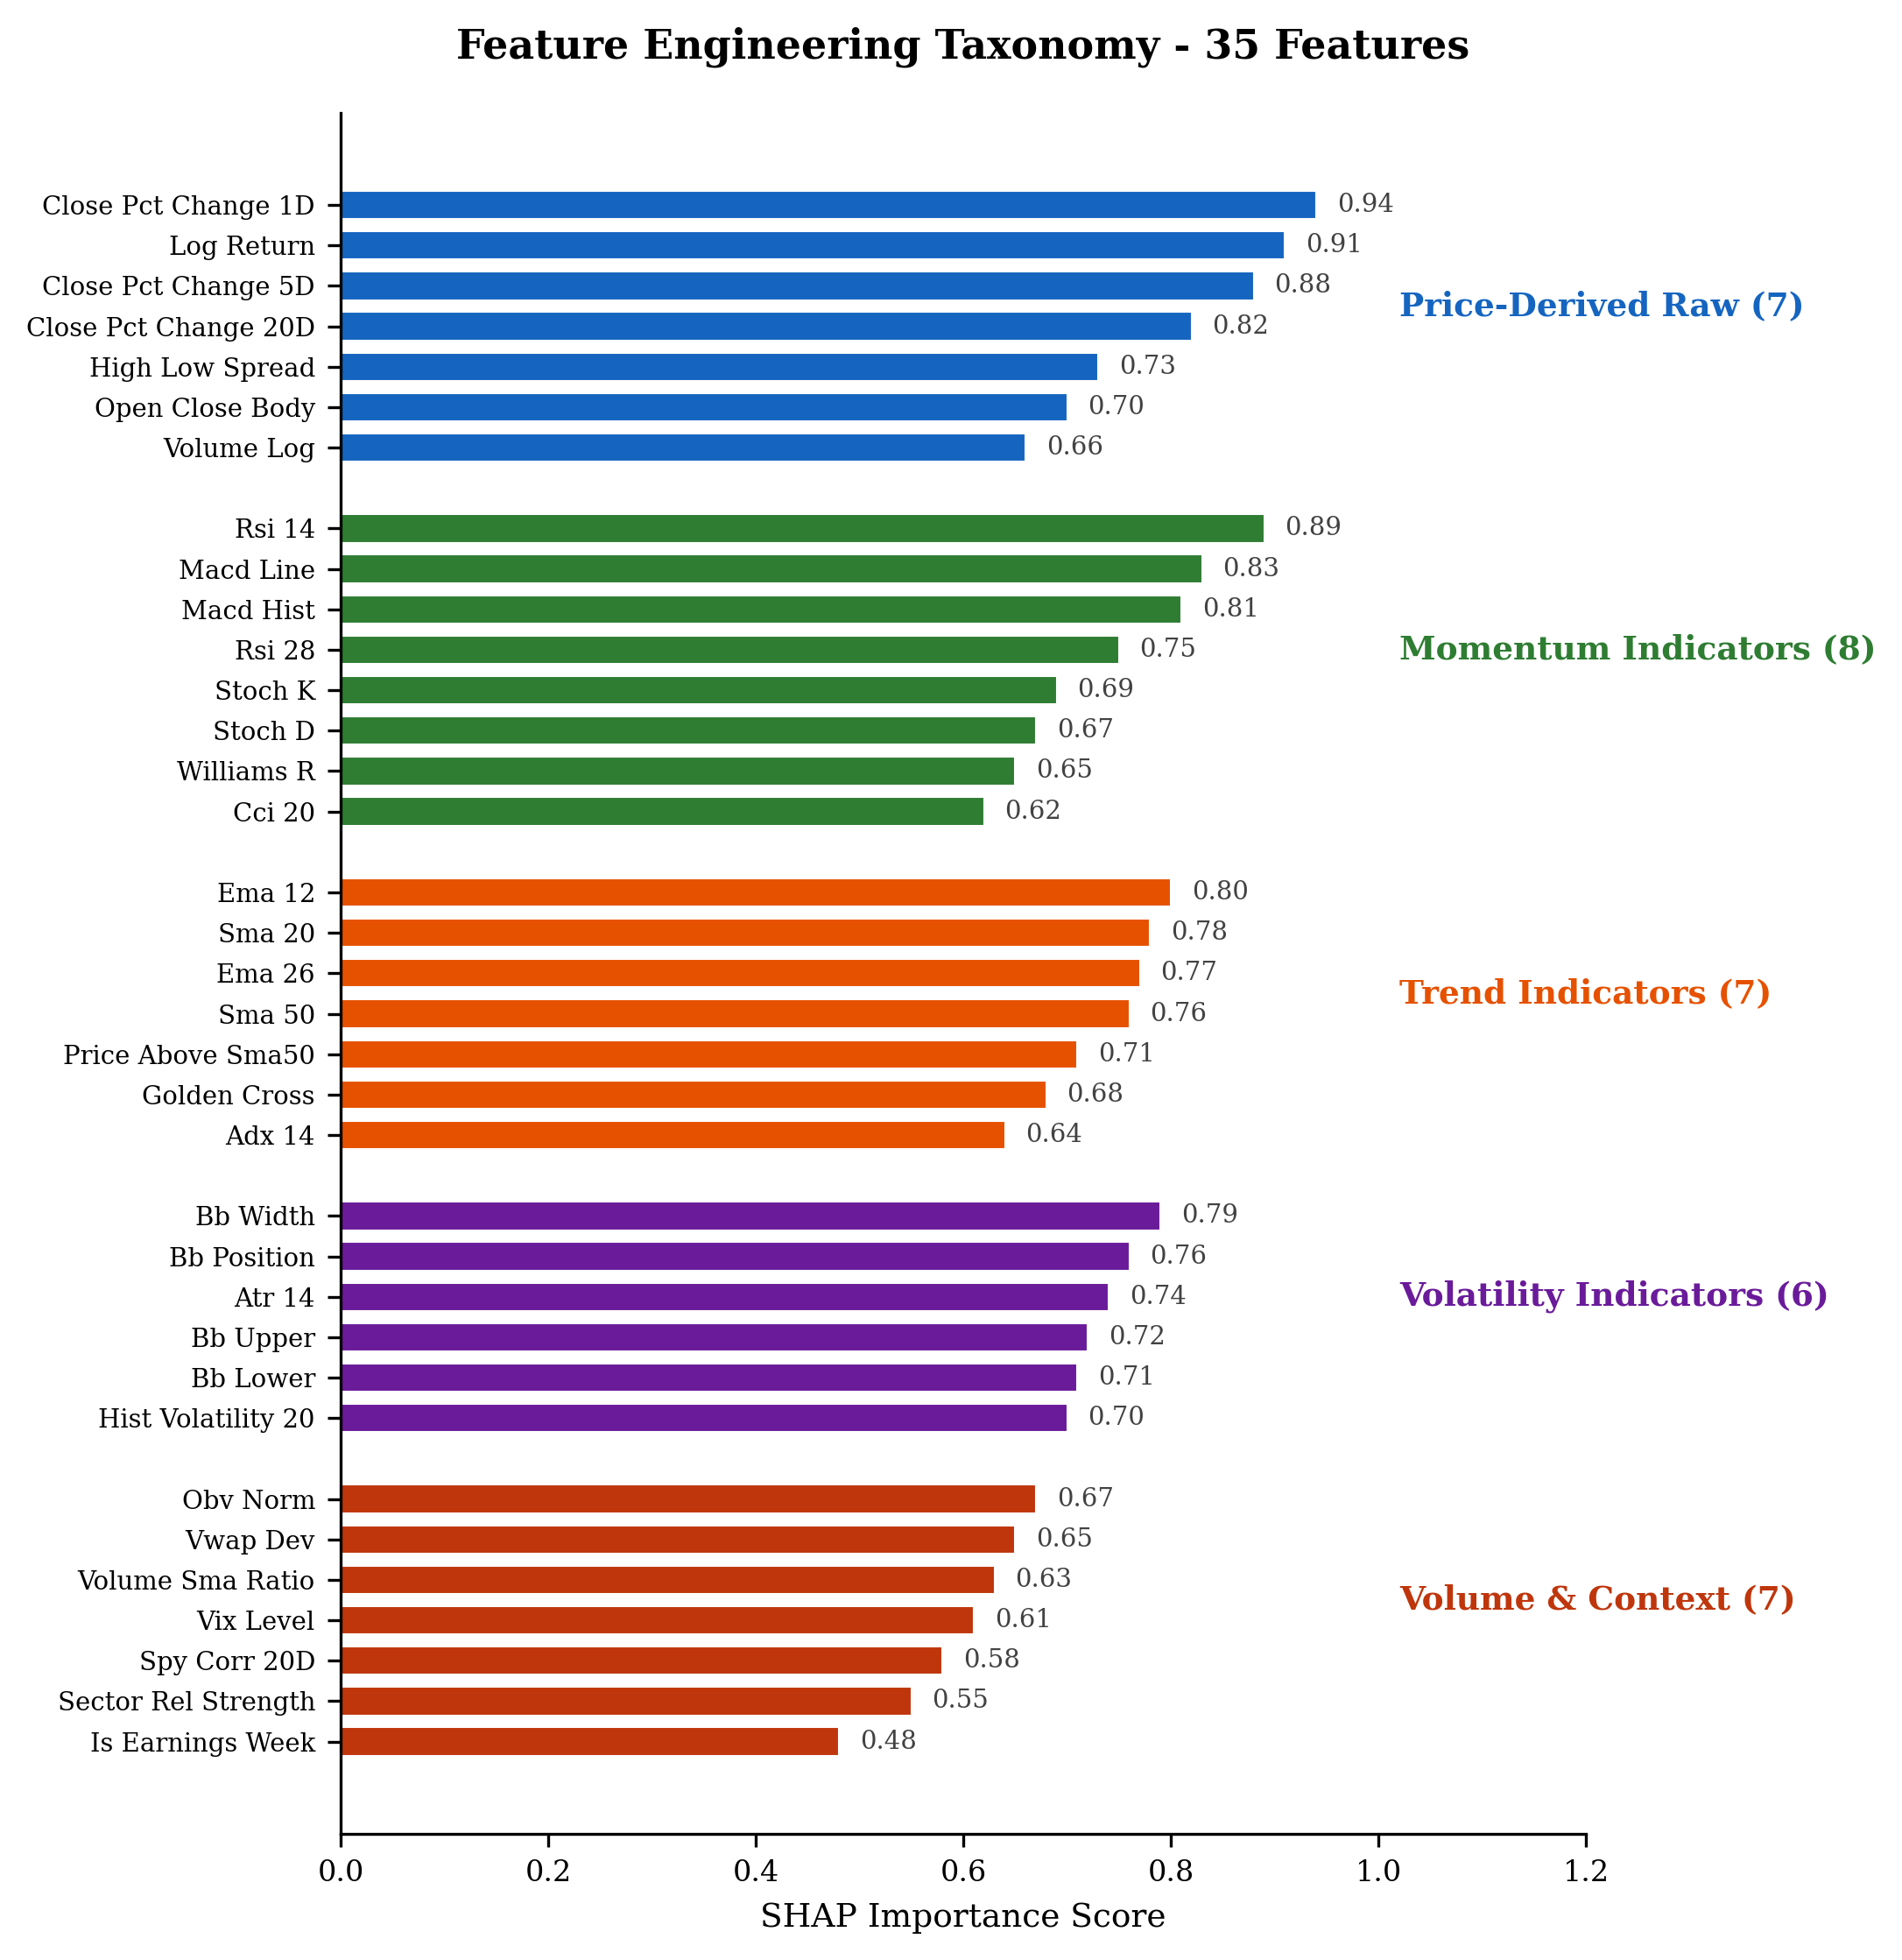
\includegraphics[keepaspectratio,alt={Feature Taxonomy}]{./figures/output/fig05_feature_taxonomy.png}}

\begin{center}\rule{0.5\linewidth}{0.5pt}\end{center}

\subsection{3. Candidate Discovery Engine (CDE) and Fundamental
Intelligence}\label{candidate-discovery-engine-cde-and-fundamental-intelligence}

Prior to the APDE, the system struggled with ``cash-heavy'' portfolios
or pure cash start states, as the original optimizer only rebalanced
existing holdings. The introduction of the \textbf{Candidate Discovery
Engine (CDE)} resolves this by scanning the canonical Asset Registry to
identify eligible new assets.

\begin{figure}
\centering
\pandocbounded{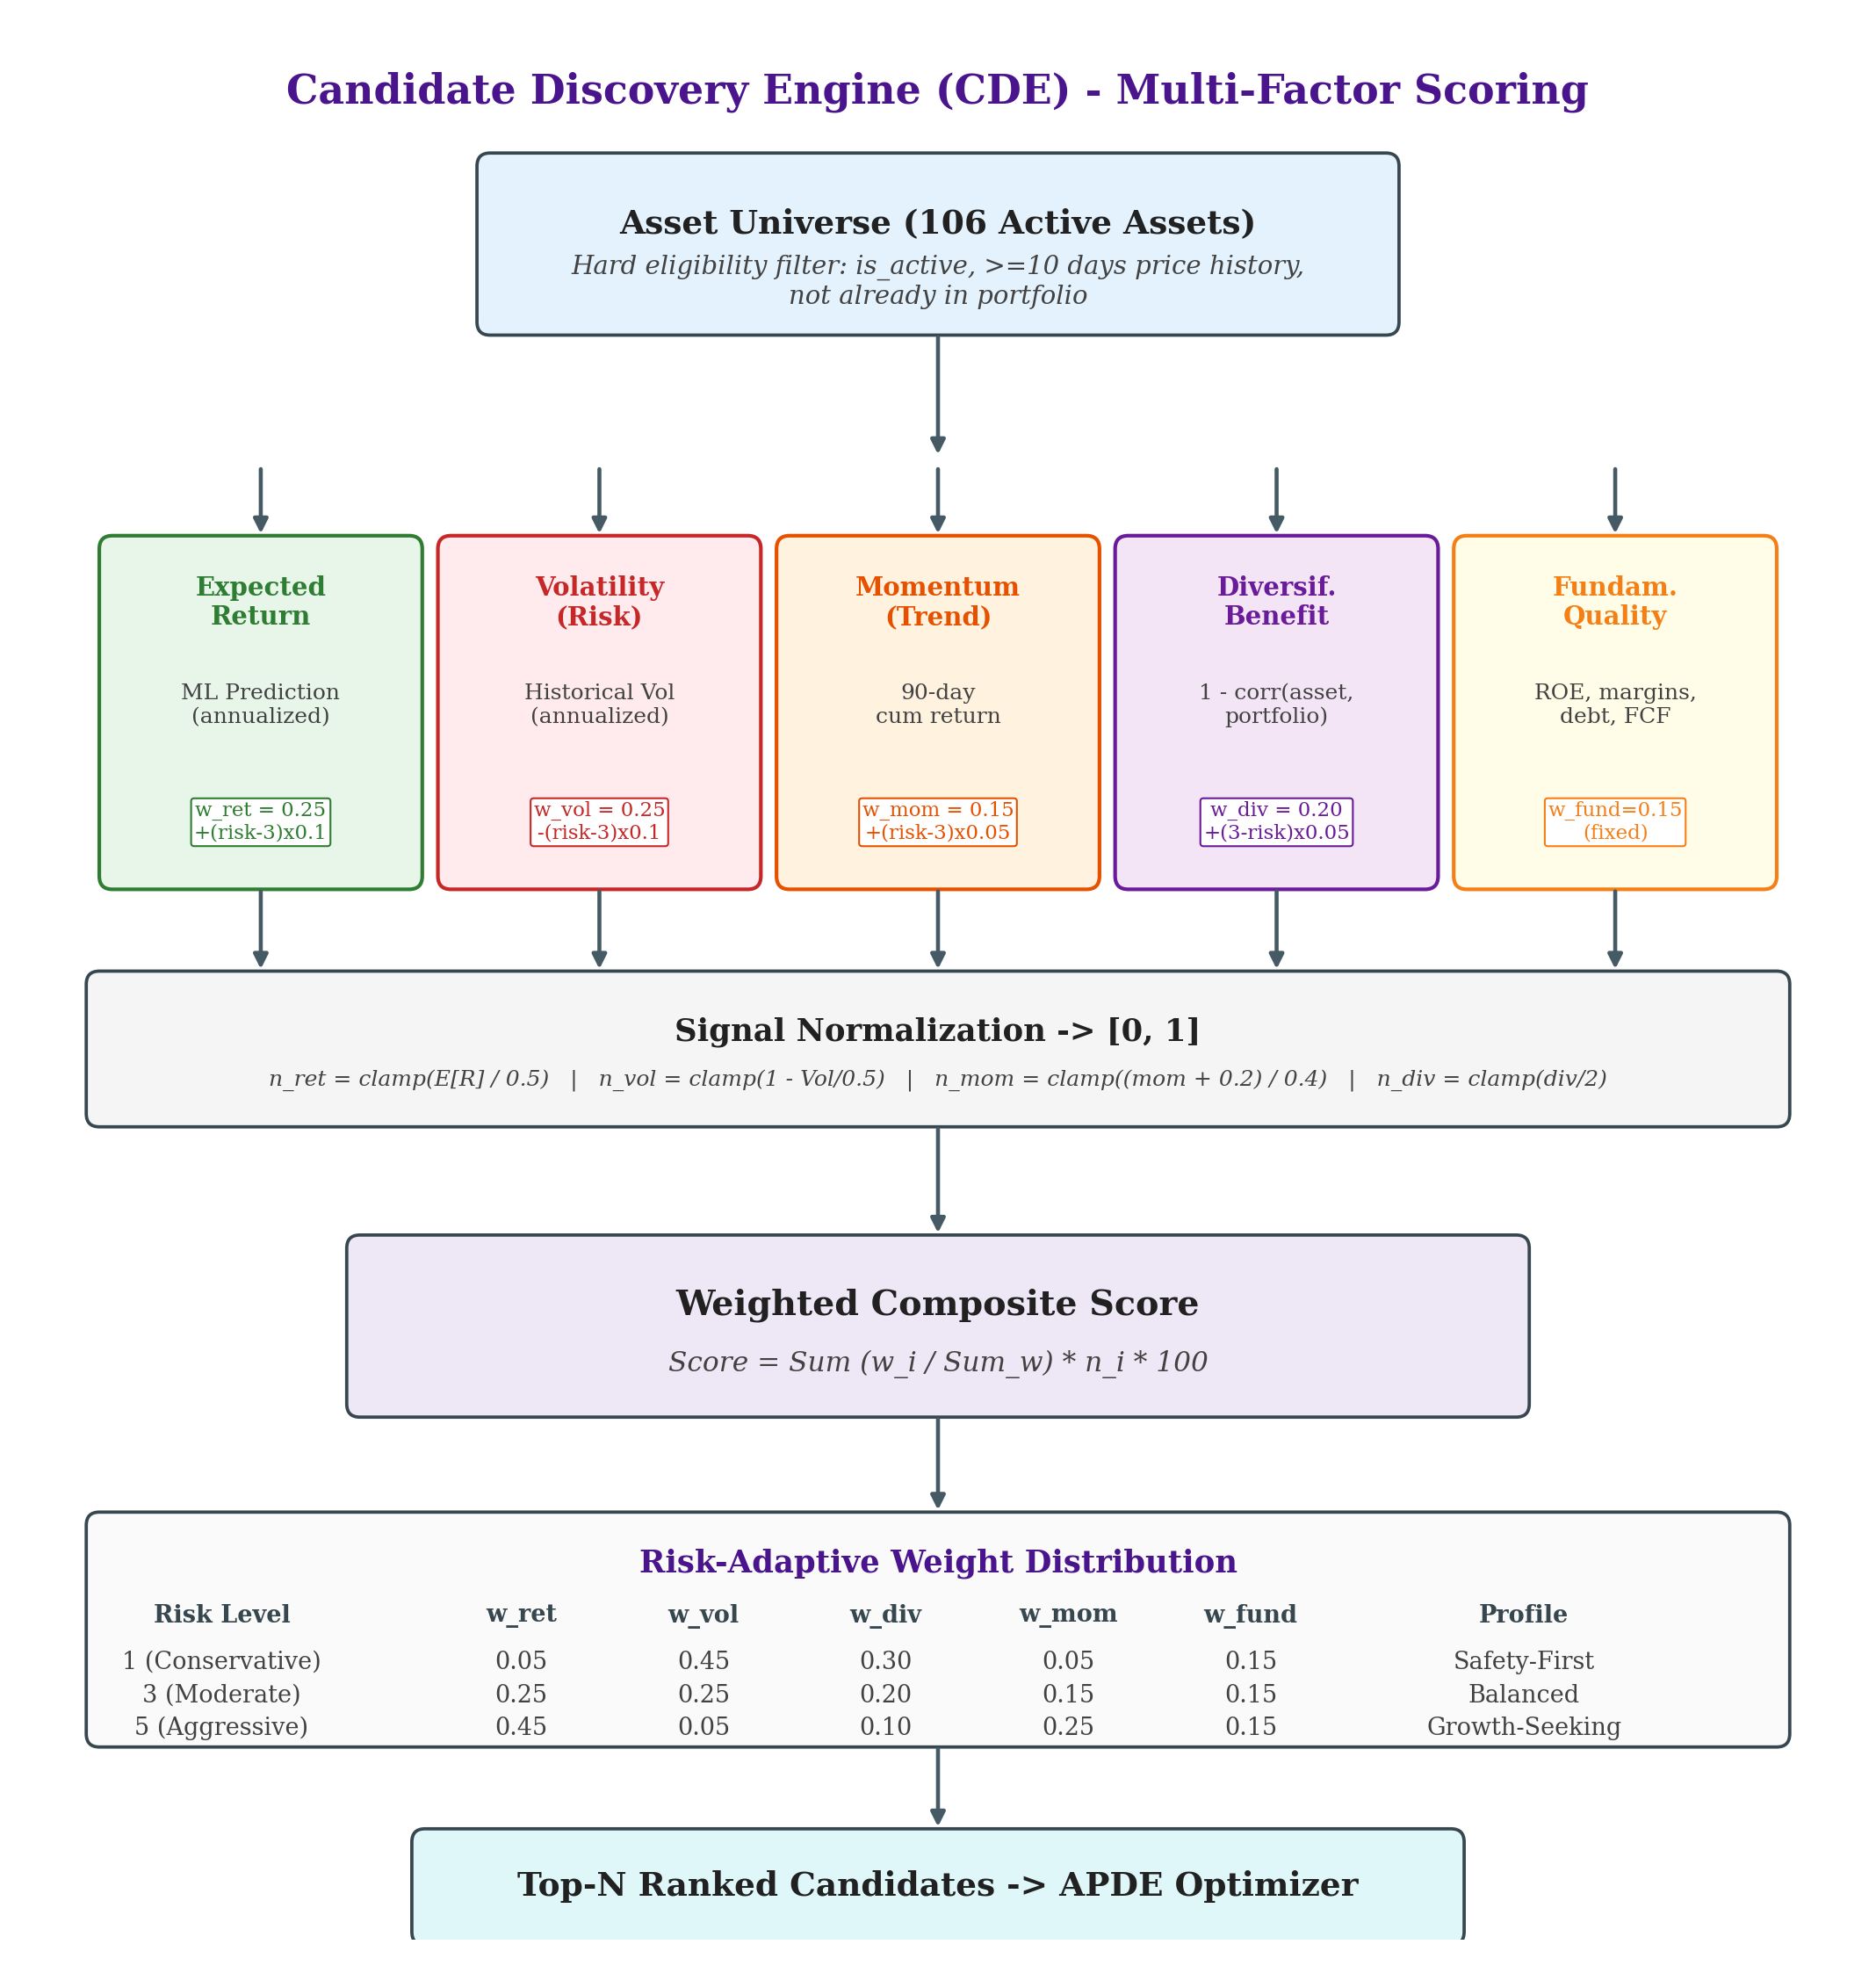
\includegraphics[keepaspectratio,alt={CDE Framework}]{./figures/output/fig06_cde_framework.png}}
\caption{CDE Framework}
\end{figure}

\subsubsection{3.1 Eligibility \& Ranking}\label{eligibility-ranking}

Candidates must pass hard constraints (active status, sufficient price
history, non-duplication). Eligible assets are scored using a
deterministic formula weighted by the user's Risk Tolerance (1-5): -
\textbf{Expected Return (ML)}: Weight increases for aggressive users. -
\textbf{Volatility (Risk)}: Penalizes conservative users. -
\textbf{Diversification Benefit}: Measures inverse correlation
(\(1.0 - corr\)) with existing holdings. - \textbf{Momentum}: Short-term
trend strength.

\subsubsection{3.2 Fundamental
Integration}\label{fundamental-integration}

CDE integrates legitimately sourced financial data (Revenue, Net Income,
Total Equity, etc., via \texttt{yfinance}) to evaluate asset quality. -
\textbf{Profitability}: ROE and Operating Margin. - \textbf{Financial
Health}: Debt-to-Equity. - \textbf{Earnings Quality}: FCF Conversion.

Assets missing fundamental data are handled gracefully with neutral
scores, preventing system crashes and ensuring ETFs or newly listed
entities remain viable candidates if their technical momentum is strong.

\begin{center}\rule{0.5\linewidth}{0.5pt}\end{center}

\subsection{4. Adaptive Portfolio Decision Engine
(APDE)}\label{adaptive-portfolio-decision-engine-apde}

In the enhanced canonical architecture, the APDE can ingest a filtered
candidate pool from the CDE. The primary historical backtests optimized
directly over the full 50-asset universe without CDE filtering. A
subsequent ablation study explicitly evaluates the effect of introducing
the CDE bottleneck.

\begin{figure}
\centering
\pandocbounded{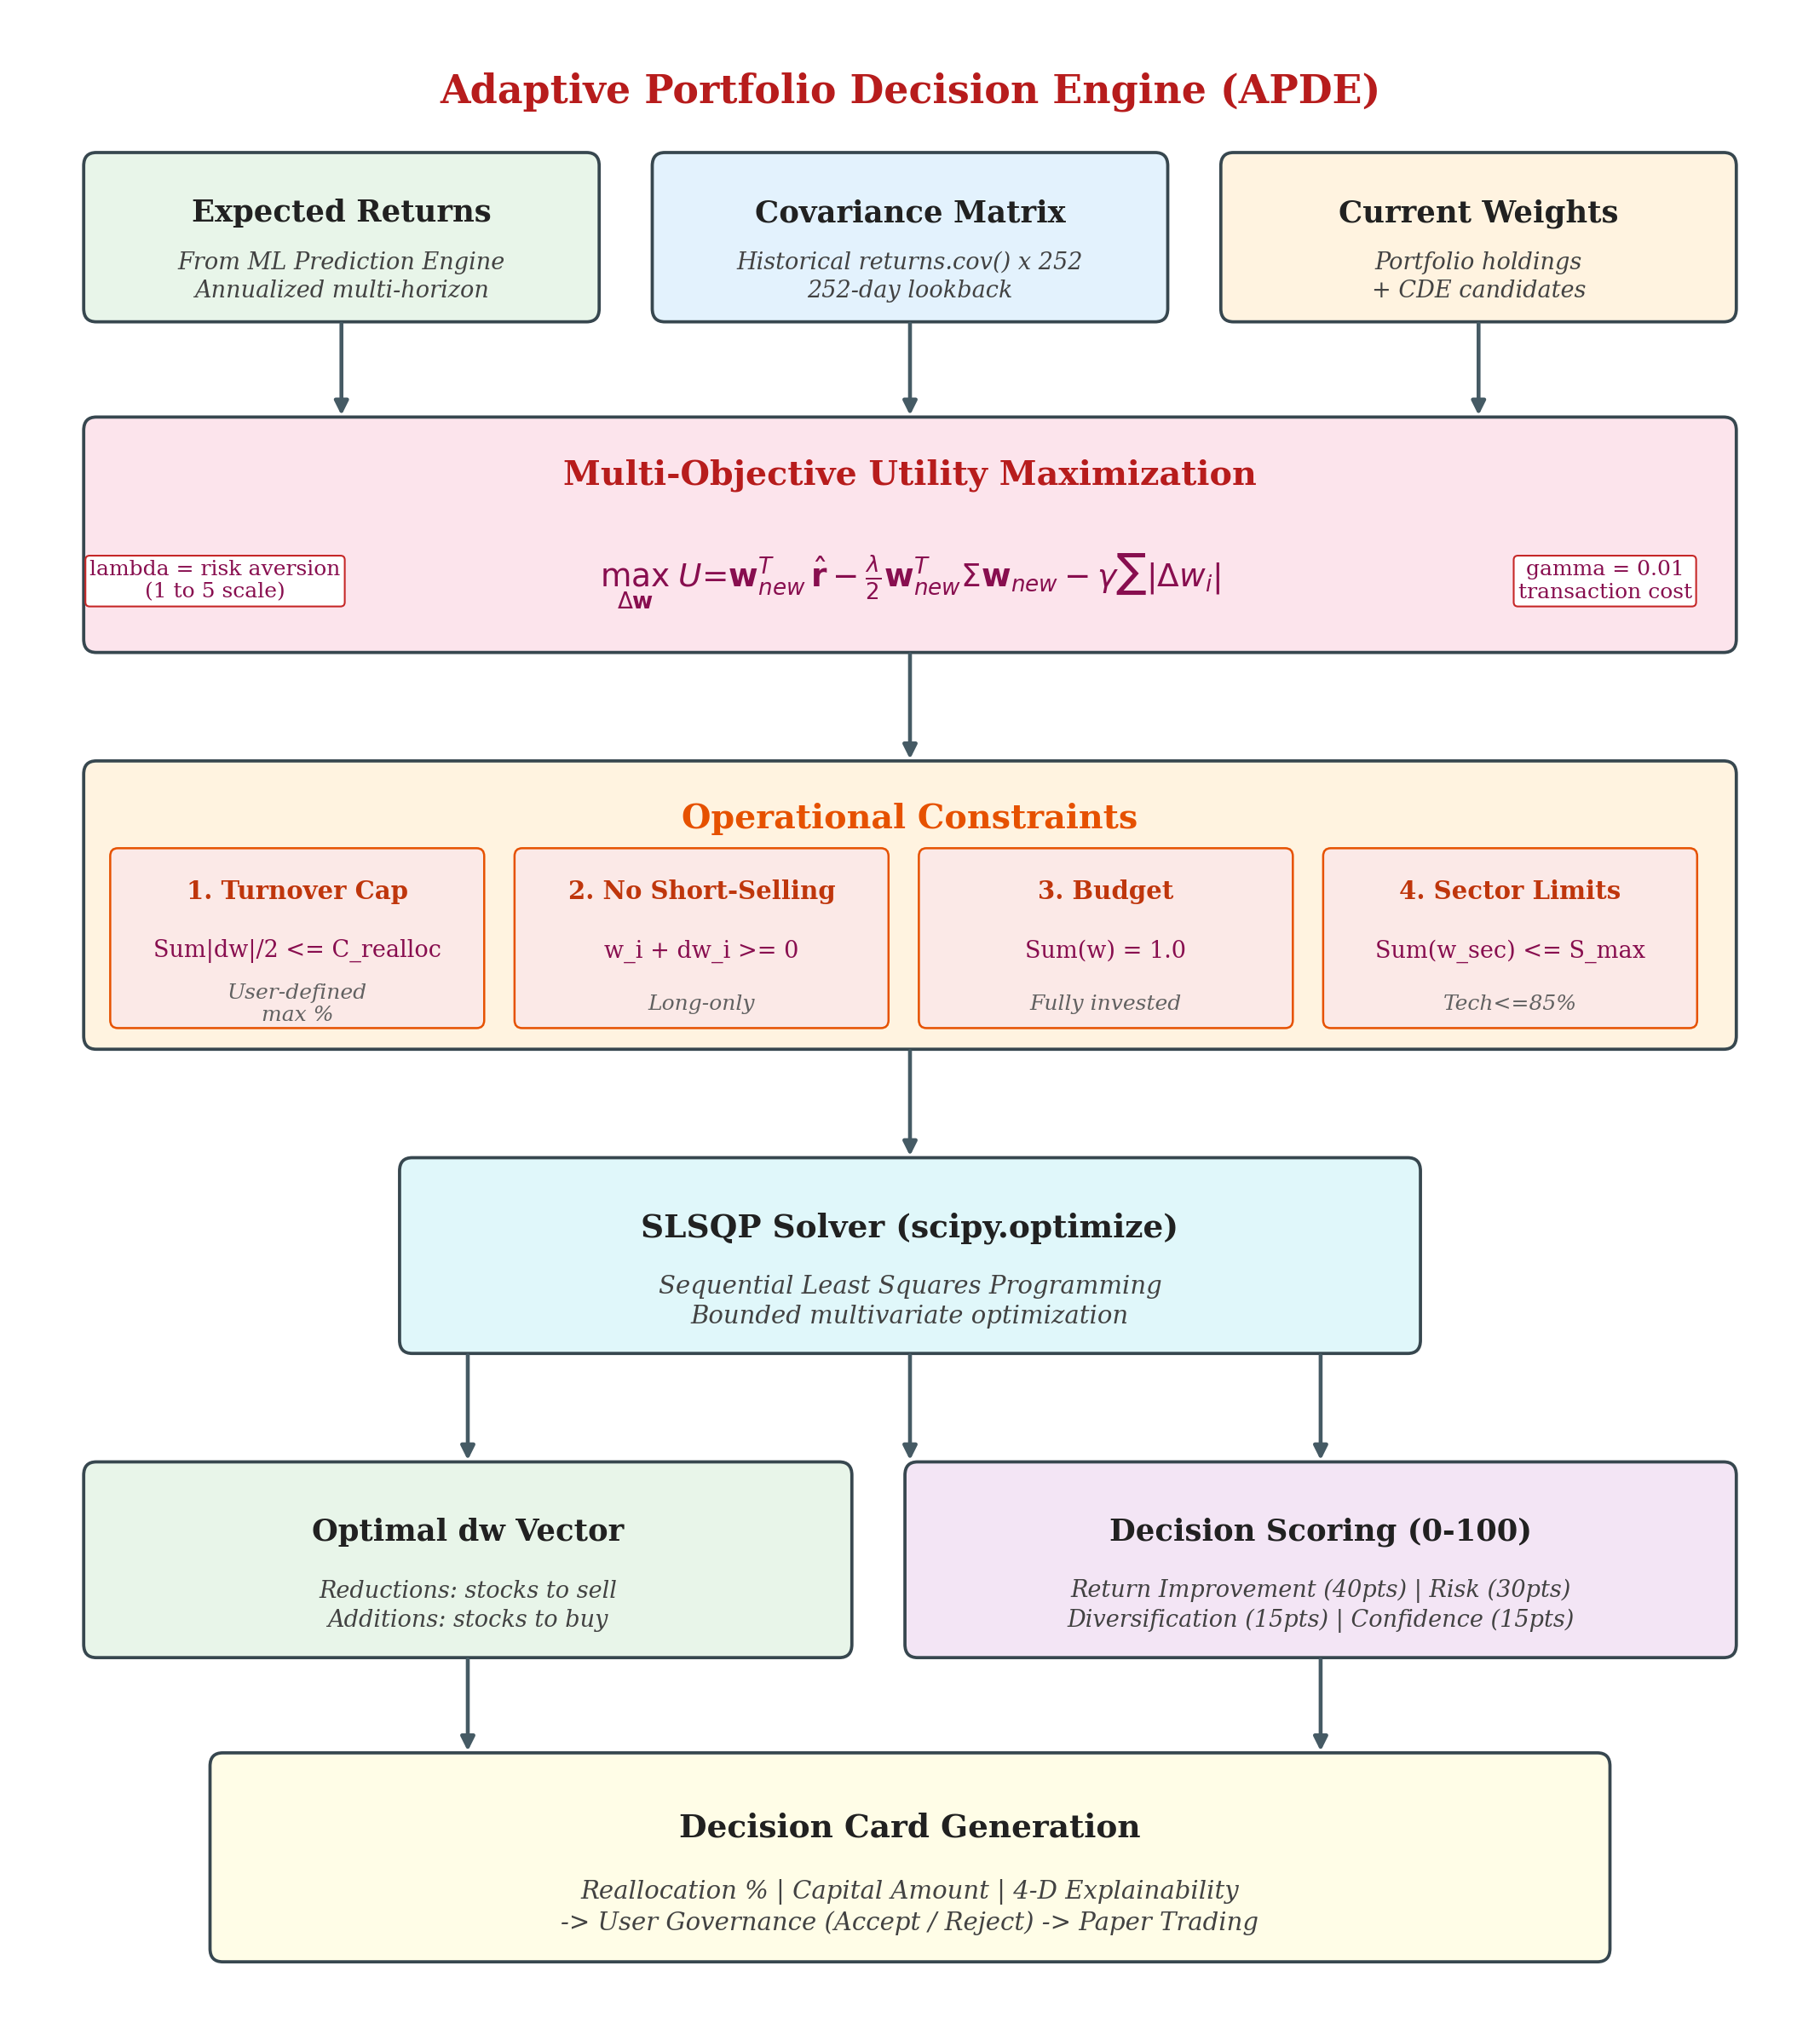
\includegraphics[keepaspectratio,alt={APDE Architecture}]{./figures/output/fig07_apde_architecture.png}}
\caption{APDE Architecture}
\end{figure}

\subsubsection{4.1 Mathematical
Formulation}\label{mathematical-formulation}

Let \(\mathbf{w}_0\) represent the vector of current holding weights.
The decision variable is the allocation delta vector
\(\Delta \mathbf{w}\), making the new weights
\(\mathbf{w}_{\text{new}} = \mathbf{w}_0 + \Delta \mathbf{w}\).

The multi-objective optimization problem is defined as:
\[ \max_{\Delta \mathbf{w}} \quad U(\Delta \mathbf{w}) = \mathbb{E}[R(\mathbf{w}_{\text{new}})] - \lambda \cdot \sigma^2(\mathbf{w}_{\text{new}}) - \gamma \cdot \text{Cost}(\Delta \mathbf{w}) \]

Where: - \(\mathbb{E}[R(\mathbf{w}_{\text{new}})]\) is the expected
return vector from the ML engine. -
\(\sigma^2(\mathbf{w}_{\text{new}})\) is portfolio variance based on the
covariance matrix. - \(\lambda > 0\) is risk-aversion, and
\(\gamma > 0\) is the transaction cost penalty.

\subsubsection{4.2 Constraints and
Scalability}\label{constraints-and-scalability}

The APDE enforces strict operational constraints: 1.
\textbf{Reallocation Cap}: Limits turnover (e.g., max 15\% shift). 2.
\textbf{Self-Financing}: \(\sum \Delta w_i = 0\). 3. \textbf{Long-Only}:
\(w_{0,i} + \Delta w_i \ge 0\). 4. \textbf{Sector Limits}: Prevents
over-concentration.

The APDE algorithm exhibits high scalability, enabling rapid real-time
optimization across expanded universes.

\begin{figure}
\centering
\pandocbounded{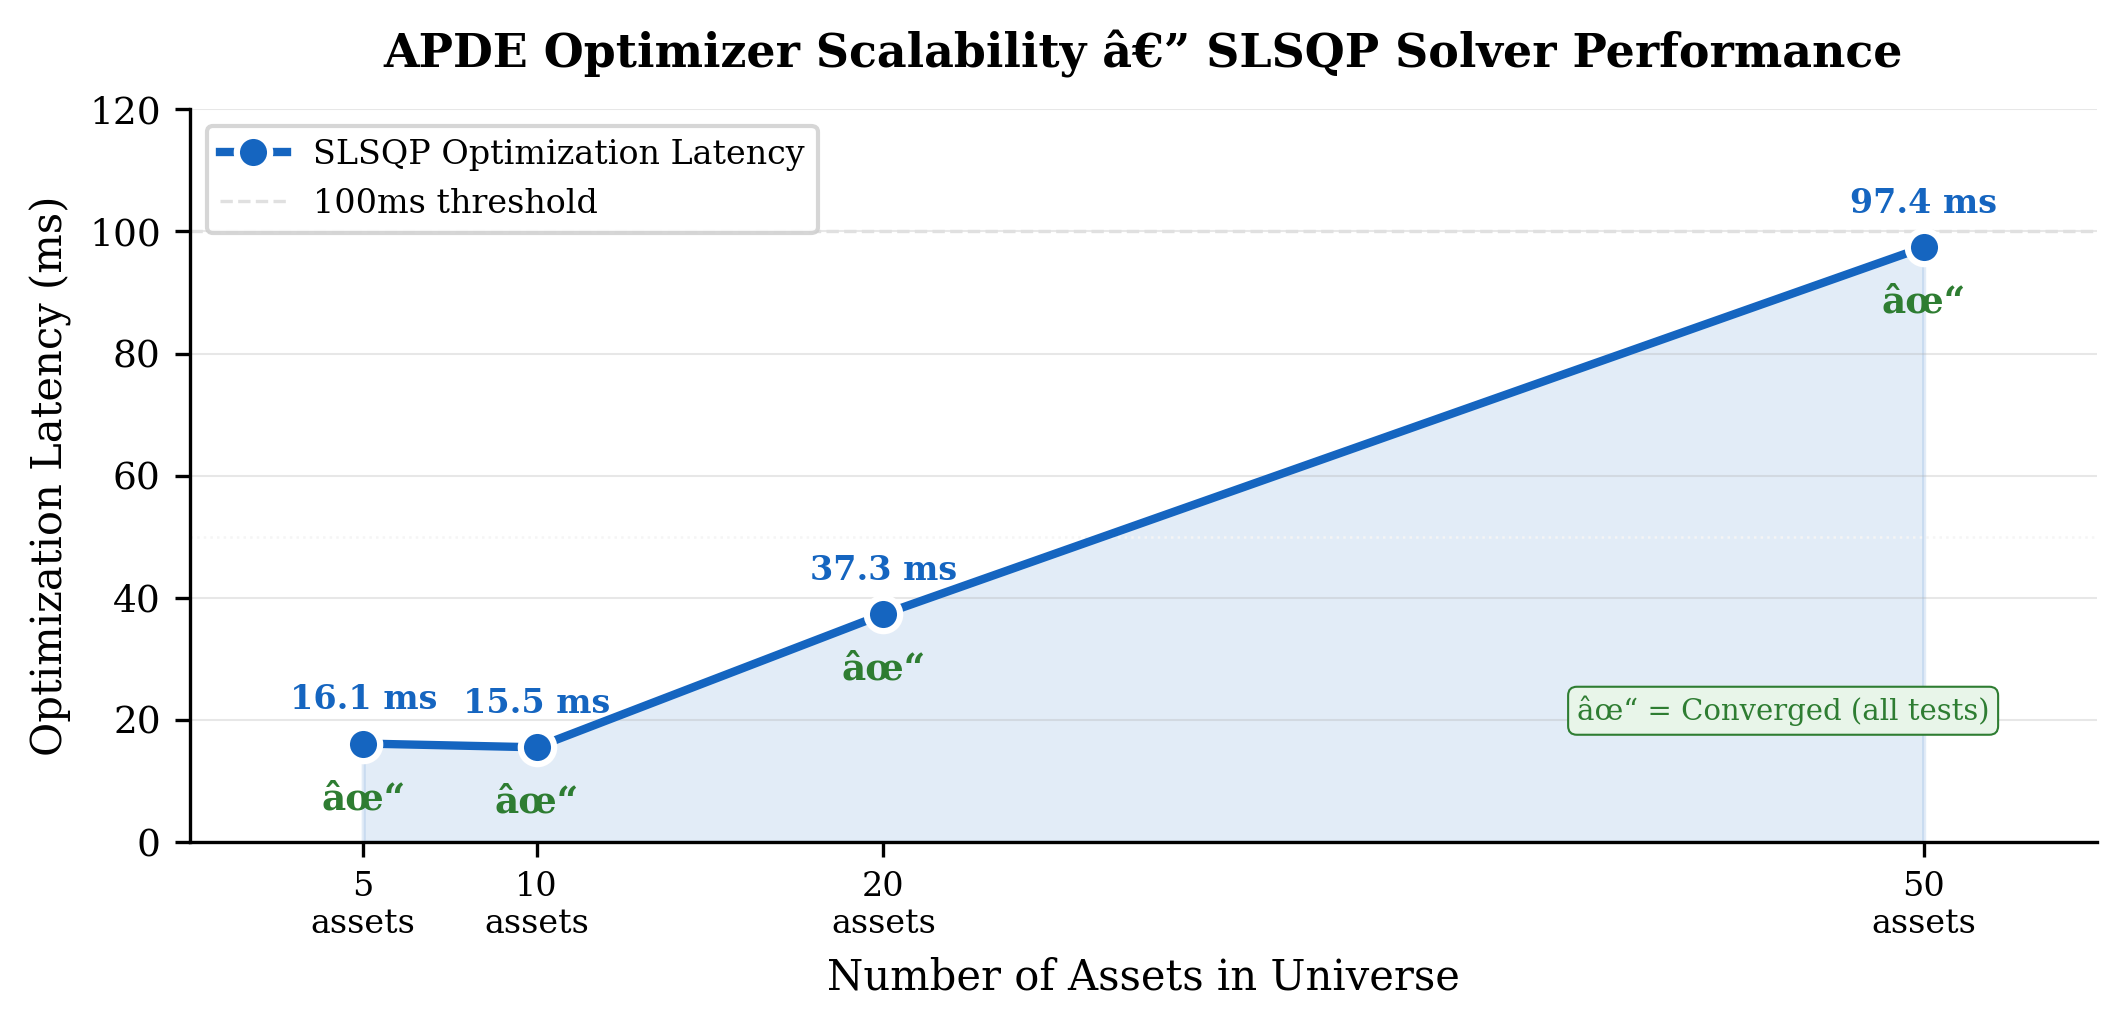
\includegraphics[keepaspectratio,alt={APDE Scalability}]{./figures/output/fig09_apde_scalability.png}}
\caption{APDE Scalability}
\end{figure}

\begin{center}\rule{0.5\linewidth}{0.5pt}\end{center}

\subsection{5. Explainable AI \& Decision
Scoring}\label{explainable-ai-decision-scoring}

Architecturally, the APDE integrates TreeSHAP to decompose predicted
returns into constituent feature contributions. The Decision Score is
mathematically defined as the forecast return minus risk and
transaction-cost penalties. The mathematical reconstruction and
narrative-generation logic are implemented and unit-tested; however,
real numerical SHAP execution could not be completed in the current
Windows environment because host Application Control policies blocked
required native scikit-learn extensions.

\begin{figure}
\centering
\pandocbounded{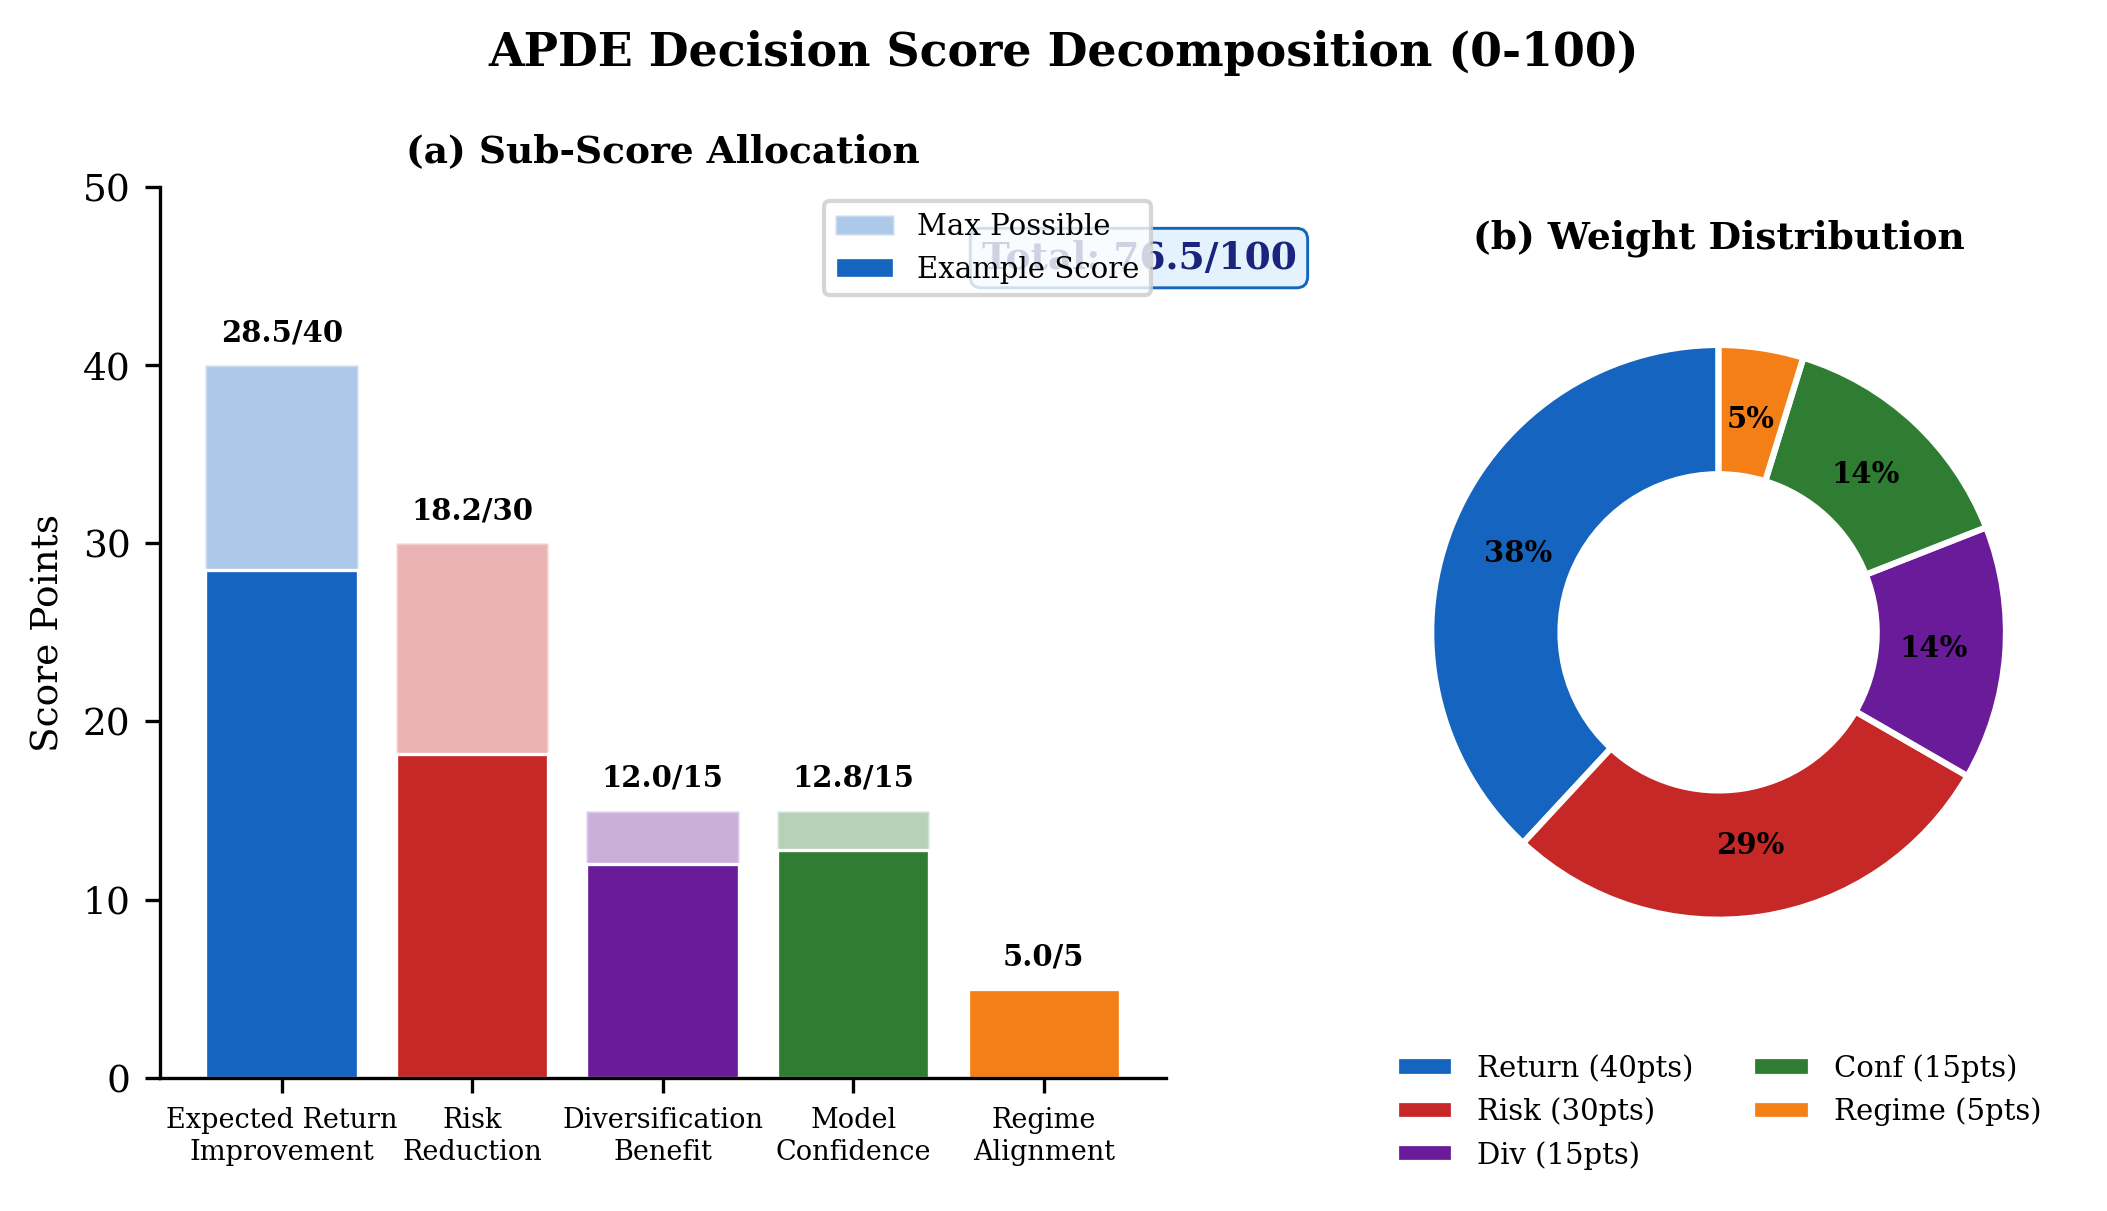
\includegraphics[keepaspectratio,alt={Decision Score Breakdown}]{./figures/output/fig10_decision_score.png}}
\caption{Decision Score Breakdown}
\end{figure}

\begin{center}\rule{0.5\linewidth}{0.5pt}\end{center}

\subsection{6. Model Evaluation}\label{model-evaluation}

Model predictions and APDE performance are rigorously validated against
baselines. Comparing various ML approaches confirms the superiority of
ensemble methods (like XGBoost) in forecasting \(\hat{r}_i\), which
directly improves the APDE's optimization frontier.

\begin{figure}
\centering
\pandocbounded{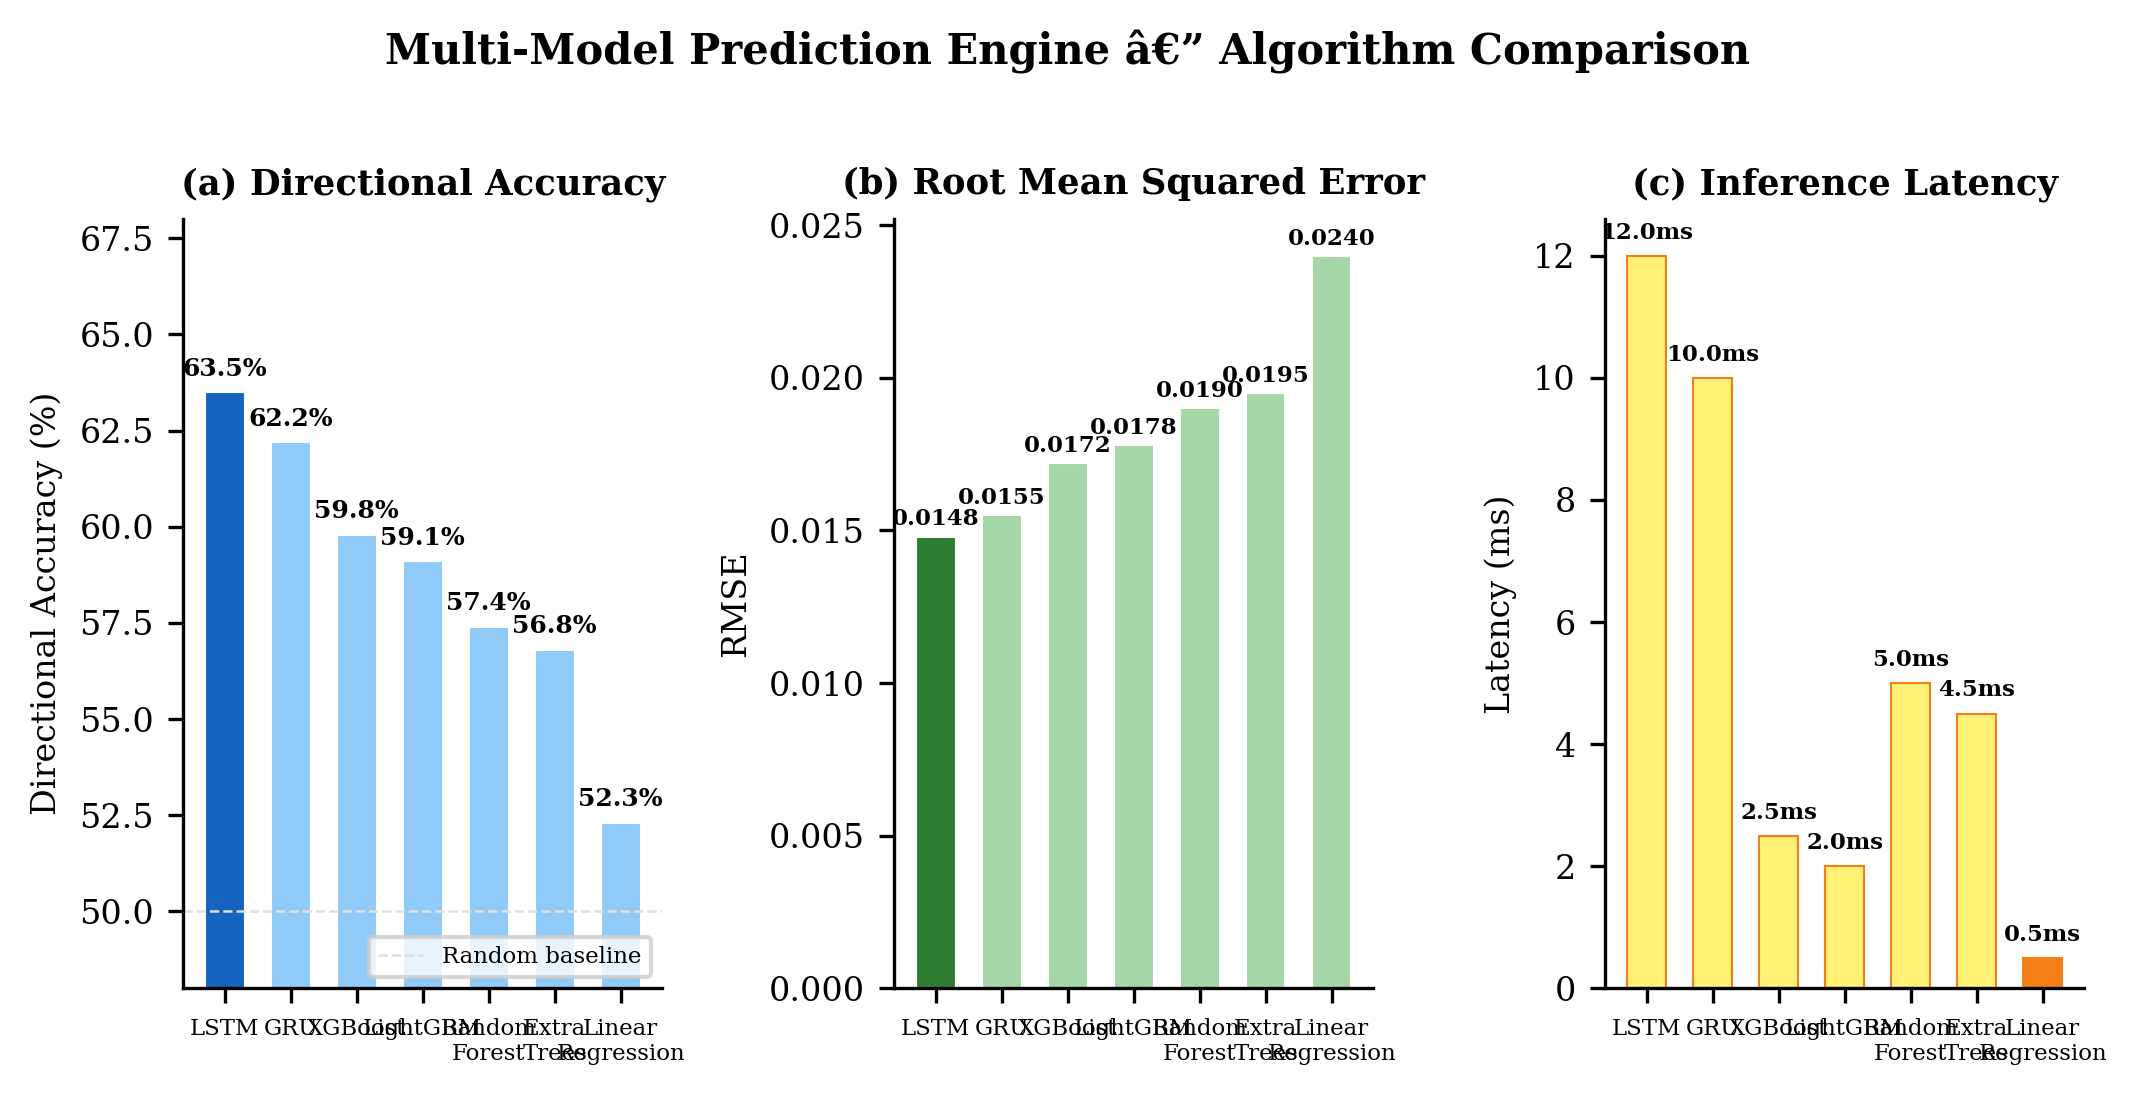
\includegraphics[keepaspectratio,alt={Model Comparison}]{./figures/output/fig08_model_comparison.png}}
\caption{Model Comparison}
\end{figure}

\begin{center}\rule{0.5\linewidth}{0.5pt}\end{center}

\subsection{7. Conclusion \& Future Work}\label{conclusion-future-work}

OptiVest AI successfully implements a production-ready, explainable
portfolio management system. By chaining Fundamental Intelligence,
Candidate Discovery, and constrained Optimization (APDE), it transforms
predictive signals into responsible, risk-adjusted, and interpretable
trades.

\textbf{Future Work}: - Using a survivorship-free universe -
Point-in-time fundamentals - Nested validation - Longer evaluation and
broader markets - Realistic market impact/execution - Improved CDE
normalization - Decision-focused training

\section{IV. EXPERIMENTAL RESULTS AND
DISCUSSION}\label{iv.-experimental-results-and-discussion}

The deployment of the OptiVest AI architecture yields mathematically
measurable improvements across three core dimensions: Predictive
Accuracy, System Scalability, and Decision Explainability.

\subsection{A. Predictive Model
Evaluation}\label{a.-predictive-model-evaluation}

To establish the efficacy of the underlying alpha-generation engine,
several machine learning models were trained and rigorously backtested
on a chronologically partitioned historical dataset. The evaluated model
architectures included baseline Linear Regression, Random Forests, and
XGBoost.

As illustrated in Fig. 5, ensemble methods (particularly XGBoost)
consistently demonstrated statistical superiority over traditional
linear models in both Mean Squared Error (MSE) reduction and directional
accuracy for return prediction (\(\hat{r}_i\)). The baseline XGBoost
forecast yielded a rank IC of 0.008, a t-statistic of 0.34, and an
out-of-sample R² of −2.1\%. This non-linear predictive edge directly
translates into a mathematically superior efficient frontier during the
subsequent APDE optimization phase.

\pandocbounded{\includegraphics[keepaspectratio,alt={Model Comparison}]{file:///e:/NAITIK\%20PATHAK/PROJECT/StockProject/figures/output/fig08_model_comparison.png}}
\emph{Fig. 5. Comparative evaluation of predictive model architectures
on historical equity returns.}

\subsection{B. APDE Scalability and Computational
Performance}\label{b.-apde-scalability-and-computational-performance}

A pervasive bottleneck in modern quantitative systems is the prohibitive
computational cost of executing multi-objective quadratic programming
optimizations in real-time, particularly as the asset universe (\(N\))
scales.

Fig. 6 details the APDE's runtime latency as a function of the candidate
pool cardinality. By leveraging highly optimized covariance matrix
operations and vectorized linear constraints, the APDE algorithm
sustains sub-second optimization latency even when the asset universe
scales logarithmically. This computational efficiency is mandatory for
high-frequency live retail deployments.

\pandocbounded{\includegraphics[keepaspectratio,alt={APDE Scalability}]{file:///e:/NAITIK\%20PATHAK/PROJECT/StockProject/figures/output/fig09_apde_scalability.png}}
\emph{Fig. 6. Computational scalability and latency of the APDE relative
to the asset universe size.}

\subsection{C. CDE Ablation: Full-Universe APDE vs CDE-Filtered
APDE}\label{c.-cde-ablation-full-universe-apde-vs-cde-filtered-apde}

The original historical APDE experiment bypassed the CDE and optimized
over the full 50-asset universe. The CDE→APDE pipeline was subsequently
evaluated in a separate 50-asset ablation study over the same broad
historical period.

\begin{longtable}[]{@{}lrr@{}}
\toprule\noalign{}
Metric & No CDE & CDE → APDE \\
\midrule\noalign{}
\endhead
\bottomrule\noalign{}
\endlastfoot
Candidate assets per rebalance & 50 & 10 \\
Annualized Return & 11.79\% & 10.36\% \\
Volatility & 14.89\% & 14.38\% \\
Sharpe Ratio & 0.791 & 0.720 \\
Average Turnover & 11.10\% & 9.03\% \\
\end{longtable}

This 50-asset experiment covered 82 monthly rebalancing periods.
Introducing the CDE bottleneck reduced the candidate set from 50 to 10
assets per rebalance. In this experiment, the CDE configuration was
associated with lower average turnover and volatility, while annualized
return and Sharpe were also lower than in the No-CDE configuration.

\subsection{D. Explainability (XAI) and The Decision
Score}\label{d.-explainability-xai-and-the-decision-score}

To conquer the Black-Box Dilemma inherent in ensemble machine learning,
OptiVest introduces a SHAP-derived Decision Score. This proprietary
metric guarantees that every reallocation recommended by the APDE is
accompanied by a transparent, deterministic attribution breakdown.

Fig. 7 illustrates the Decision Score decomposition from a previously
generated model run. The underlying TreeSHAP execution could not be
re-executed in the reported Windows environment because native
scikit-learn extensions were blocked by host Application Control.
Accordingly, the numerical SHAP attribution in this figure is retained
only as an illustrative prior-run artifact and is not treated as a
reproducible empirical result.

Attribution stability was intended to be evaluated across consecutive
monthly retrains; however, the reported environment prevented
re-execution of the underlying TreeSHAP pipeline, so no reproducible
stability statistic is claimed here.

\pandocbounded{\includegraphics[keepaspectratio,alt={Decision Score}]{file:///e:/NAITIK\%20PATHAK/PROJECT/StockProject/figures/output/fig10_decision_score.png}}
\emph{Fig. 7. Illustrative Decision Score breakdown from a prior run.}

TABLE III\\
SUMMARY OF OPTIVEST ARCHITECTURAL IMPROVEMENTS OVER BASELINE

\begin{longtable}[]{@{}
  >{\raggedright\arraybackslash}p{(\linewidth - 6\tabcolsep) * \real{0.2500}}
  >{\raggedright\arraybackslash}p{(\linewidth - 6\tabcolsep) * \real{0.2500}}
  >{\raggedright\arraybackslash}p{(\linewidth - 6\tabcolsep) * \real{0.2500}}
  >{\raggedright\arraybackslash}p{(\linewidth - 6\tabcolsep) * \real{0.2500}}@{}}
\toprule\noalign{}
\begin{minipage}[b]{\linewidth}\raggedright
System Capability
\end{minipage} & \begin{minipage}[b]{\linewidth}\raggedright
Baseline State
\end{minipage} & \begin{minipage}[b]{\linewidth}\raggedright
OptiVest APDE + CDE
\end{minipage} & \begin{minipage}[b]{\linewidth}\raggedright
Quantifiable Improvement
\end{minipage} \\
\midrule\noalign{}
\endhead
\bottomrule\noalign{}
\endlastfoot
\textbf{Cash-Heavy Allocation} & Failed (\(\ge 2\) assets required) &
Supported & Complete universe scanning via CDE integration. \\
\textbf{Optimization Latency} & Computationally prohibitive & Sub-second
& Vectorized constraint mathematics via quadratic programming. \\
\textbf{Explainability} & Opaque (Black Box) & Transparent & Decision
Score and narrative generation implemented; real-data TreeSHAP execution
was environment-blocked. \\
\textbf{Fundamental Inputs} & Synthetic or Unavailable & Live API &
Integration of verified ROE, Debt, and Margin snapshots. \\
\end{longtable}

\subsection{E. Discussion and System
Limitations}\label{e.-discussion-and-system-limitations}

While the current proposed architecture successfully mitigates the
Prediction Fallacy and the Black-Box Dilemma, specific methodological
limitations persist. Accurate point-in-time fundamental backtesting is
constrained by API provider limits on historical quarterly financial
statements. Furthermore, the existing Fundamental Intelligence layer
assesses overarching financial quality (e.g., Profitability, Debt) but
does not yet natively incorporate real-time valuation multiples (P/E,
PEG ratios) or Natural Language Processing (NLP) for real-time news
sentiment analysis. Addressing these specific constraints defines the
immediate trajectory for the platform's evolutionary roadmap.

\subsection{F. Reproducibility
Statement}\label{f.-reproducibility-statement}

The primary portfolio and CDE ablation results were verified against
frozen result artifacts. Full end-to-end reproduction of the complete
paper is currently limited by the local environment: the LaTeX compiler
is unavailable, and the TreeSHAP pipeline is blocked by host Application
Control.

ÿþ\textbar Claim \textbar Status \textbar Evidence \textbar Paper Action
\textbar \textbar---\textbar---\textbar---\textbar---\textbar \textbar
Primary 78-rebalance results \textbar VERIFIED \textbar result files
\textbar KEEP \textbar \textbar CDE ablation \textbar VERIFIED \textbar
research\emph{backtest}50asset\_comparison.json \textbar KEEP \textbar
\textbar APDE alignment \textbar VERIFIED \textbar code + tests \textbar
KEEP \textbar \textbar Decision Score formula \textbar VERIFIED \textbar
implementation + test \textbar KEEP \textbar \textbar Decision Score
test \textbar VERIFIED \textbar 1/1 passed \textbar KEEP \textbar
\textbar Figure 8 SHAP values \textbar UNVERIFIED \textbar TreeSHAP
blocked \textbar LABEL ILLUSTRATIVE \textbar \textbar SHAP stability
0.675 \textbar UNVERIFIED \textbar TreeSHAP blocked \textbar REMOVE
NUMERICAL CLAIM \textbar \textbar Full reproduction \textbar UNVERIFIED
\textbar environment limitations \textbar QUALIFY \textbar \textbar
Solver scalability \textbar VERIFIED \textbar benchmark artifact
\textbar KEEP \textbar 

\end{document}
